\documentclass[tikz,border=0pt]{standalone}
\usepackage{graphicx}
\usepackage{sansmath}
\usetikzlibrary{arrows.meta,calc}
\definecolor{PtArrow}{HTML}{777386}
\definecolor{GeArrow}{HTML}{1E5E5C}
\definecolor{Ink}{HTML}{333B40}
\definecolor{TOCBackground}{HTML}{F0F5F4}
\begin{document}
\sansmath
\begin{tikzpicture}[x=1cm,y=1cm,
  every node/.style={font=\sffamily\fontsize{8.5}{10}\selectfont,text=Ink},
  movement/.style={line width=0.6pt,line cap=round,-{Stealth[length=1.15mm,width=0.8mm]}},
  leader/.style={line width=0.5pt,line cap=round}]
  \path[use as bounding box] (0,0) rectangle (8,3);
  \fill[TOCBackground] (0,0) rectangle (8,3);

  % Faint background cluster motifs; the main reaction remains in front.
  \node[inner sep=0pt,opacity=0.30] at (0.45,2.55) {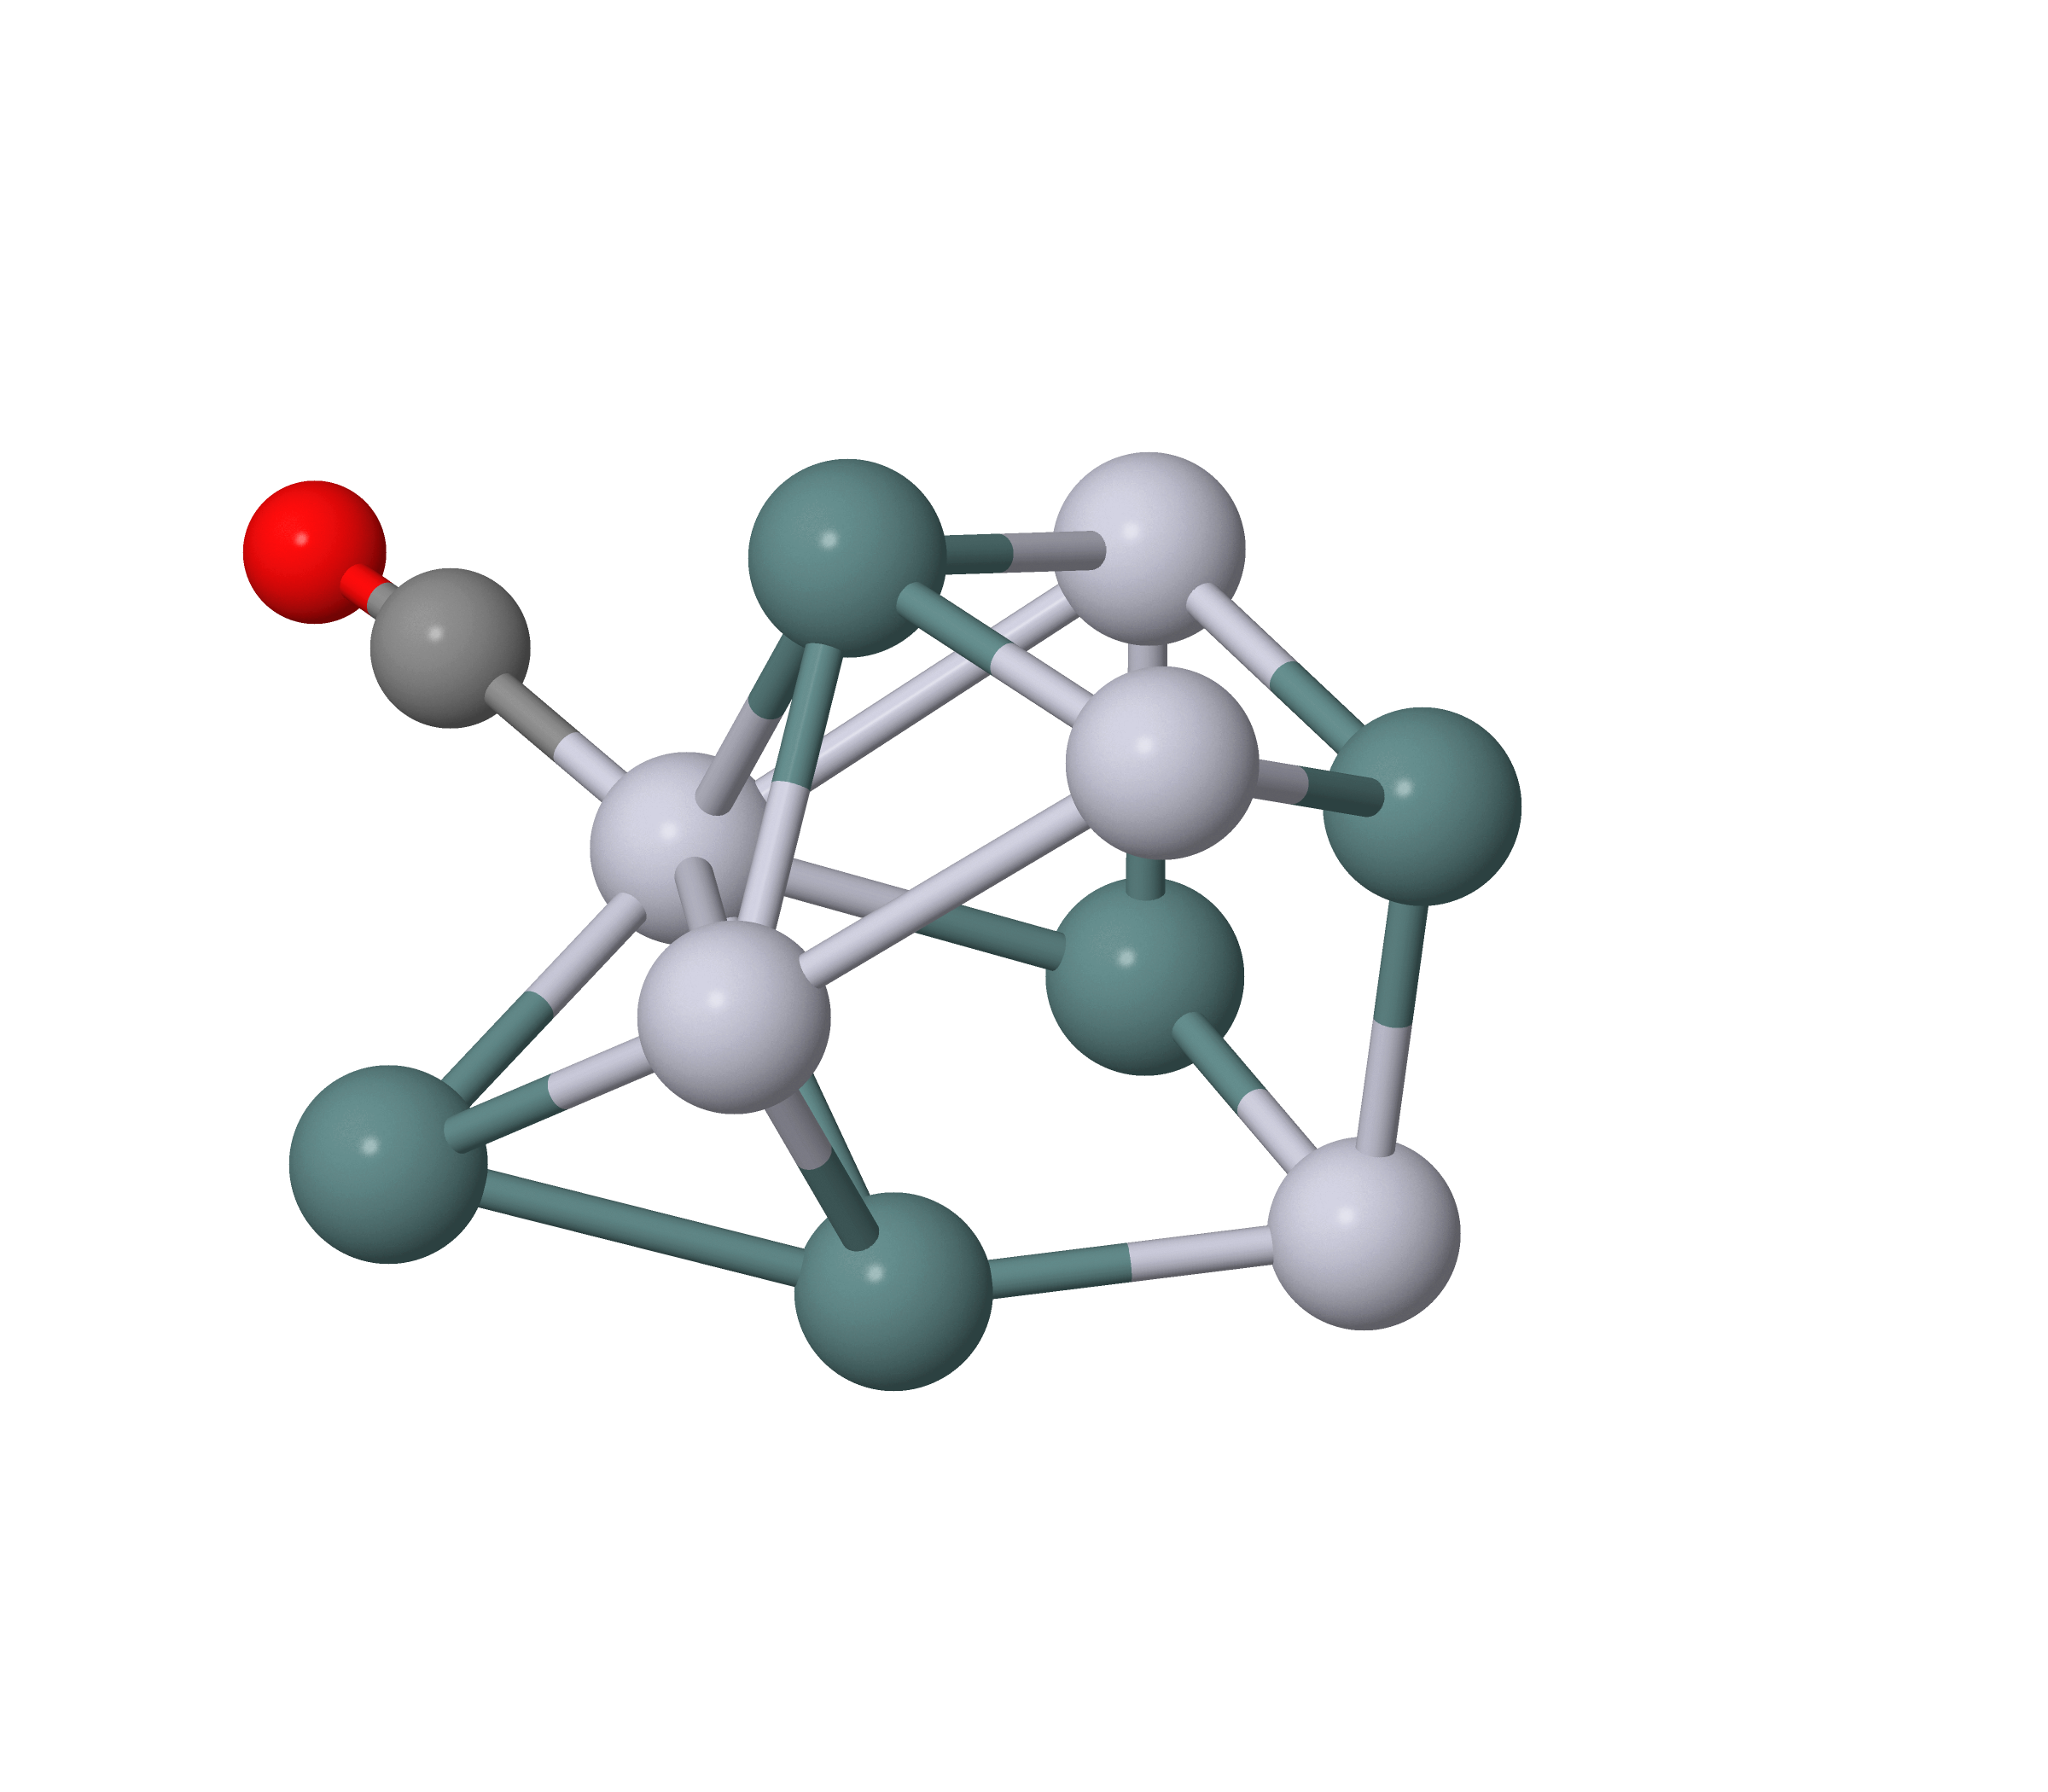
\includegraphics[width=0.72cm]{c7.png}}; %1
  \node[inner sep=0pt,opacity=0.30] at (1.88,0.82) {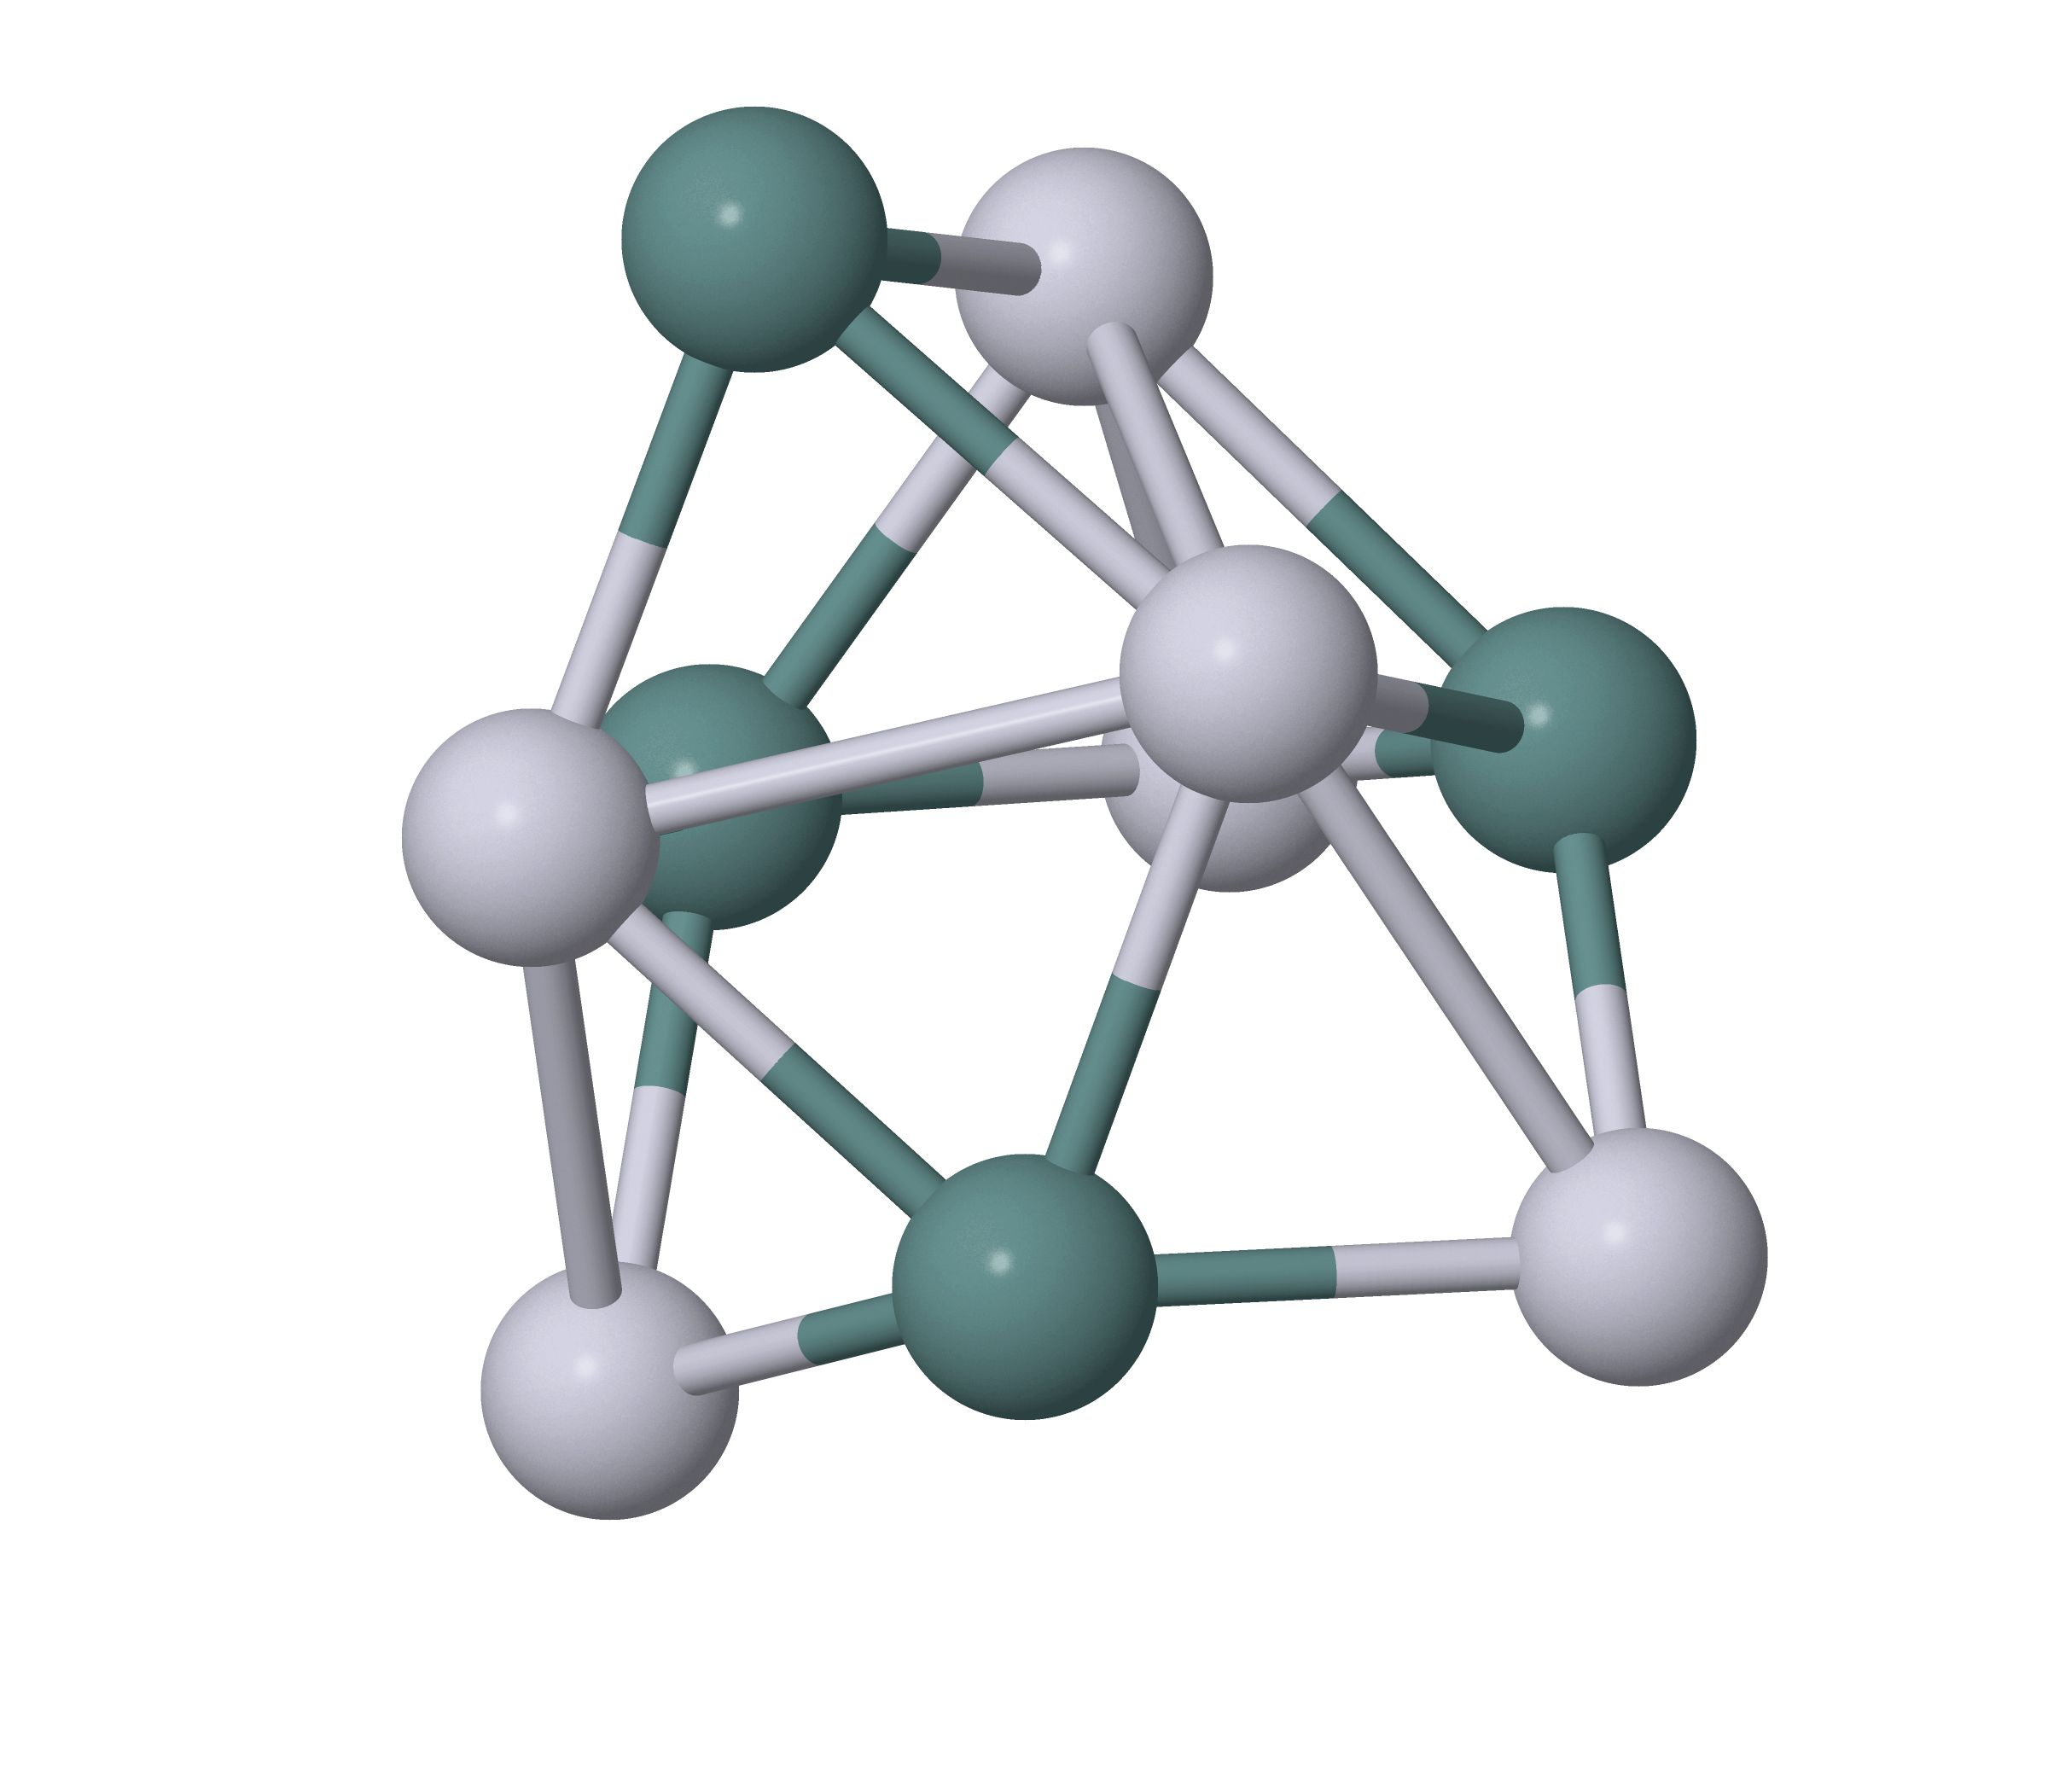
\includegraphics[width=0.68cm]{c2.png}};  %2
  \node[inner sep=0pt,opacity=0.30] at (2.08,2.12) {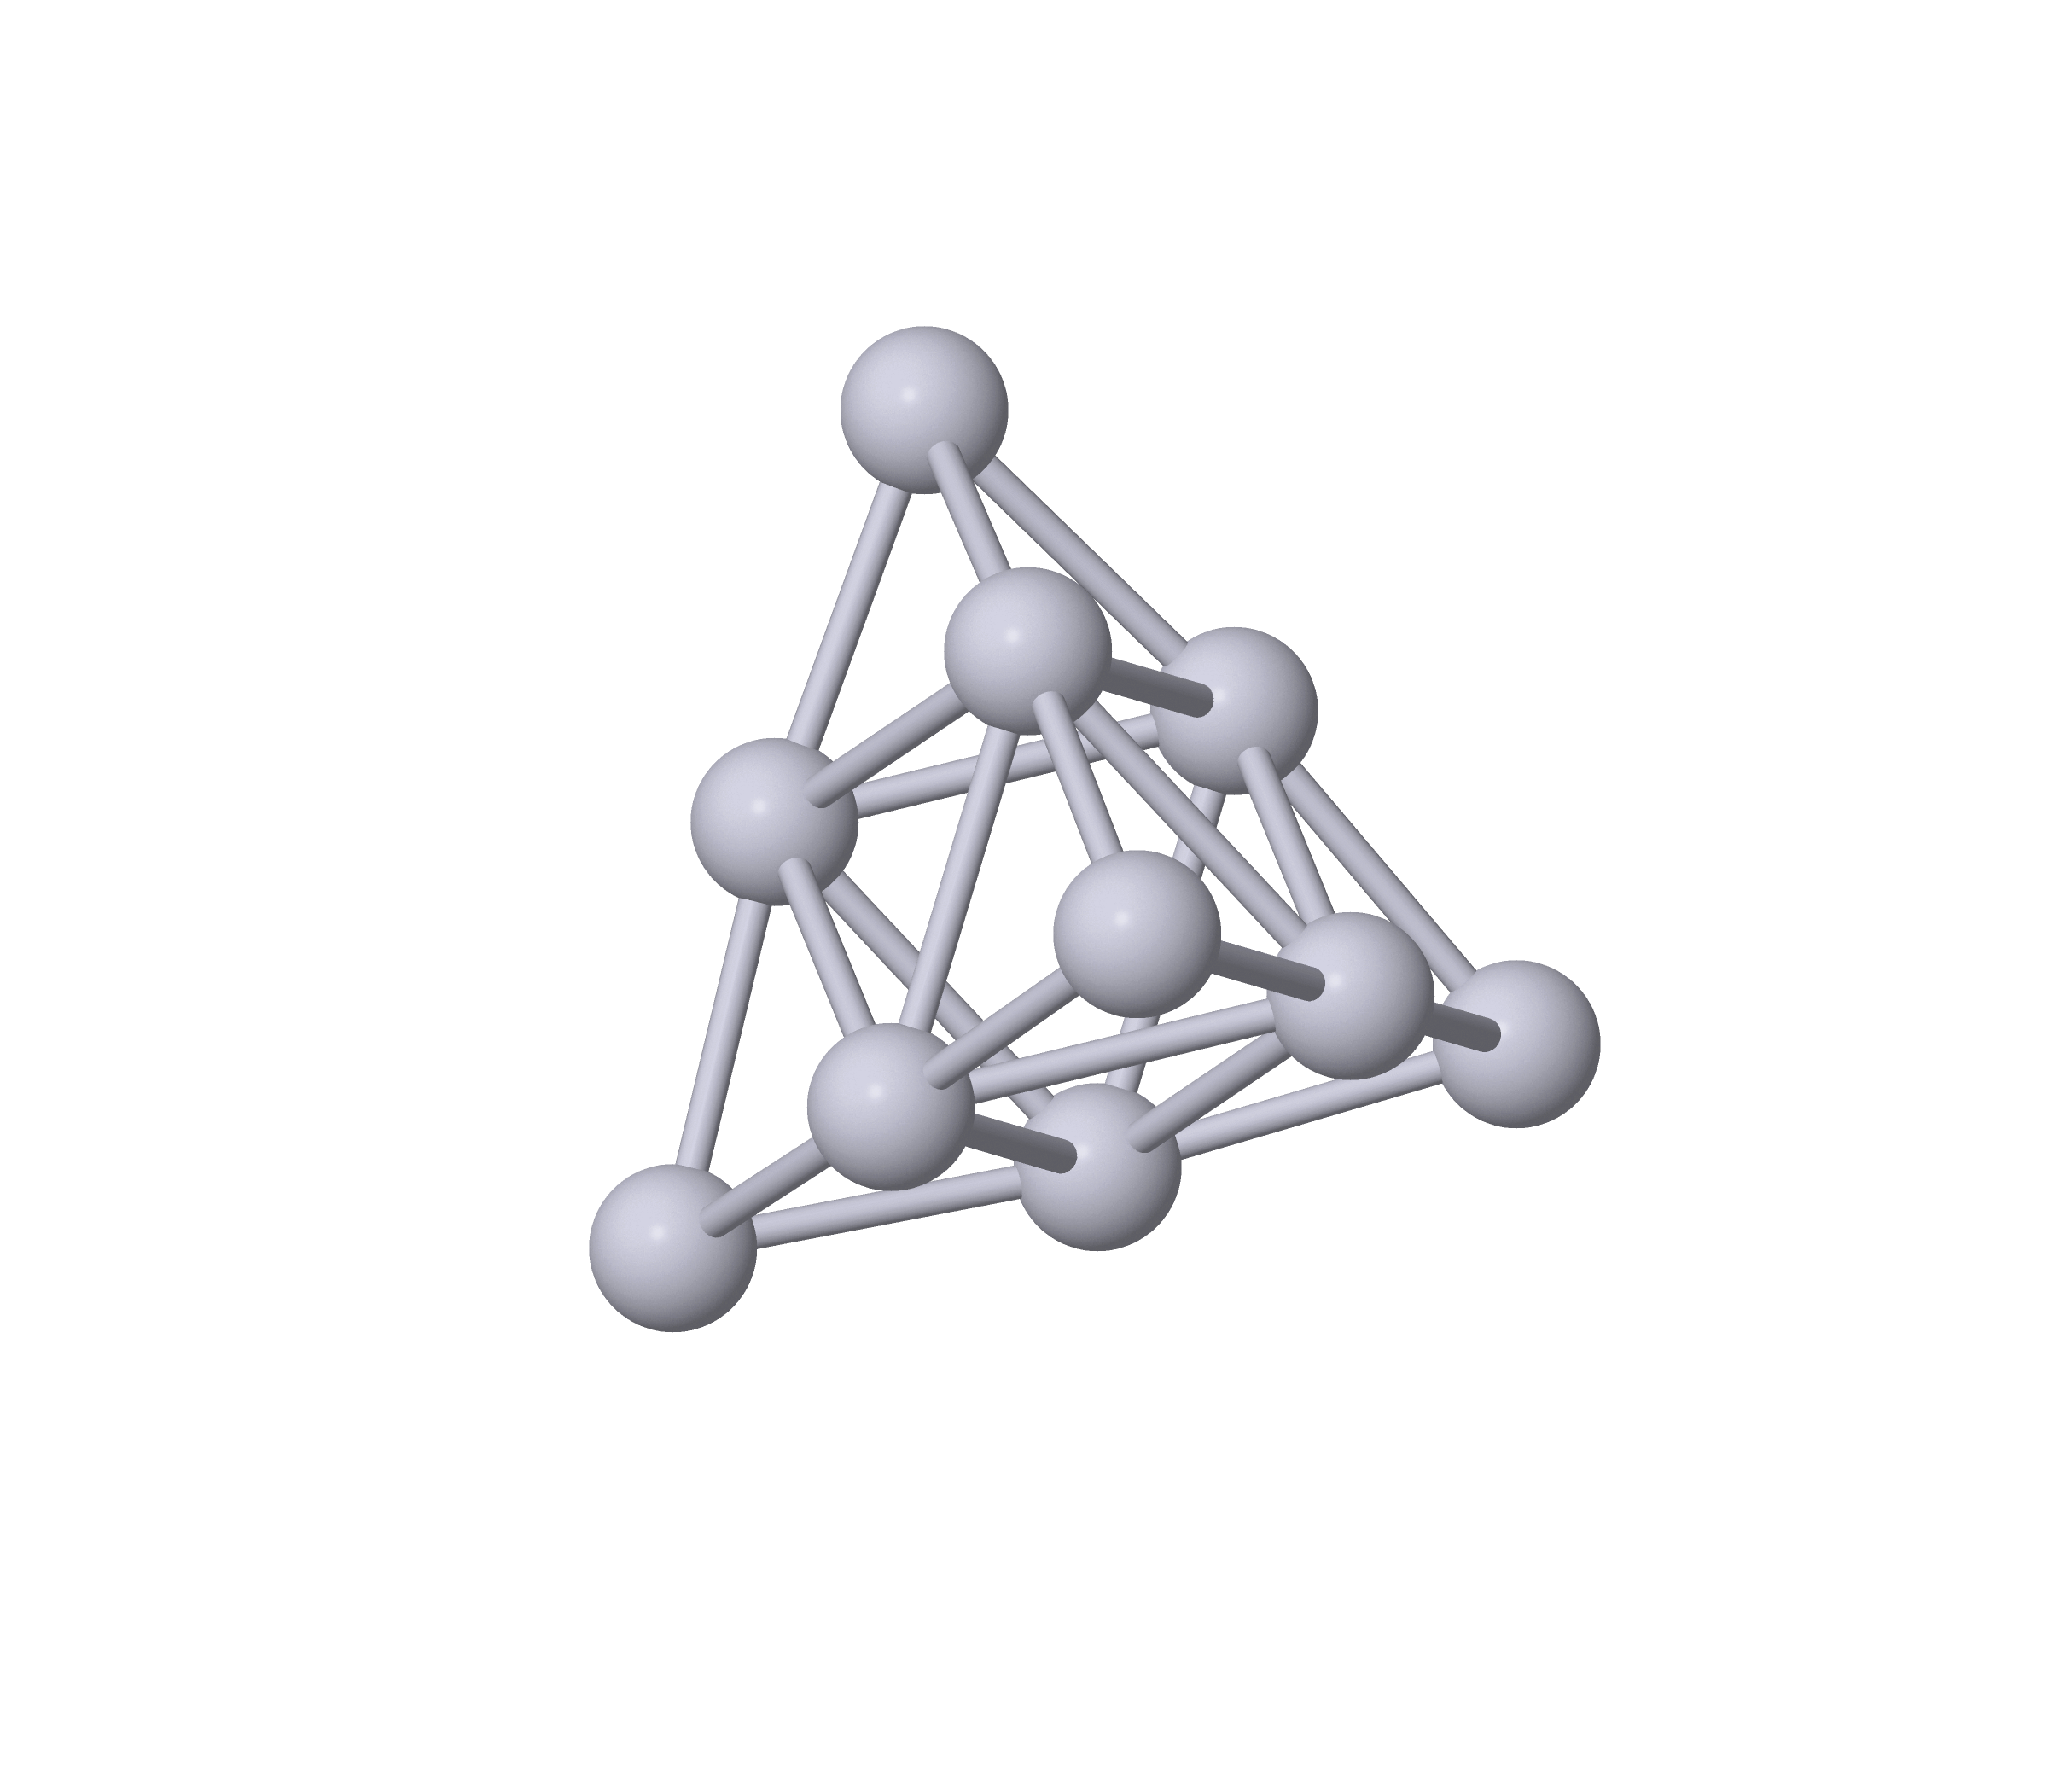
\includegraphics[width=0.8cm,angle=90.0]{c5.png}};  %2
  \node[inner sep=0pt,opacity=0.32] at (2.95,2.40) {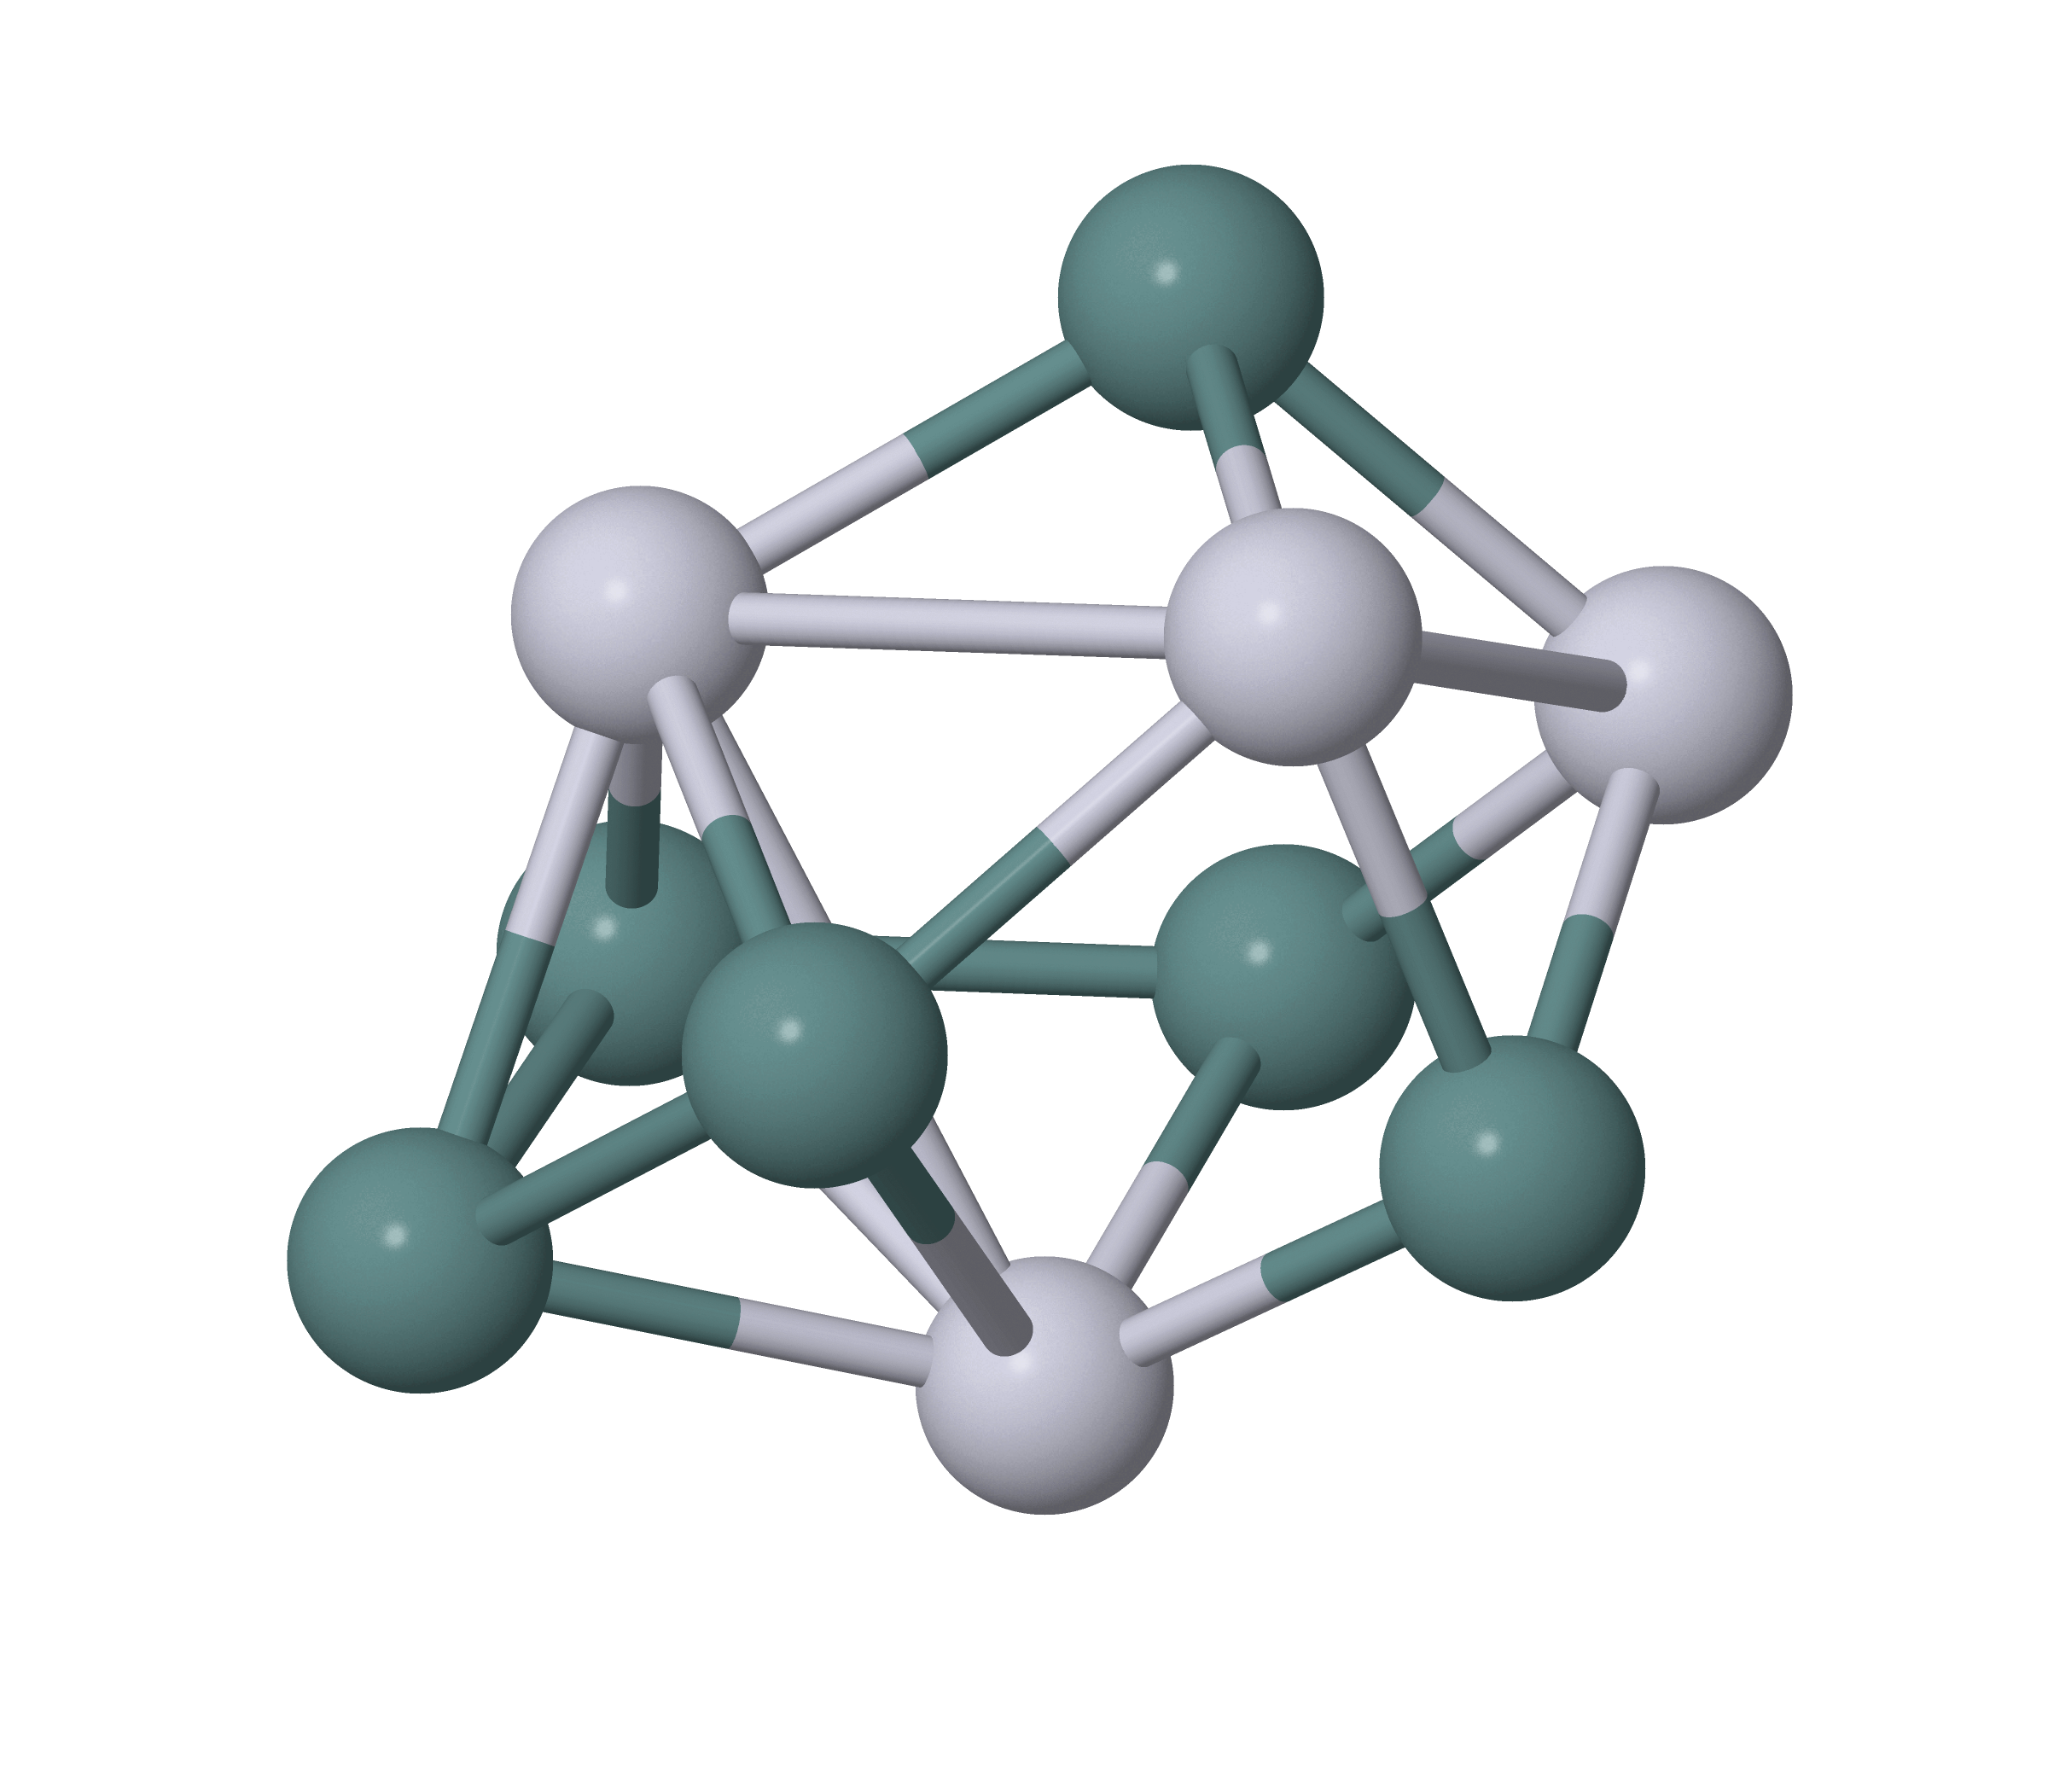
\includegraphics[width=0.68cm]{c3.png}};  %3
  \node[inner sep=0pt,opacity=0.30] at (3.52,0.34) {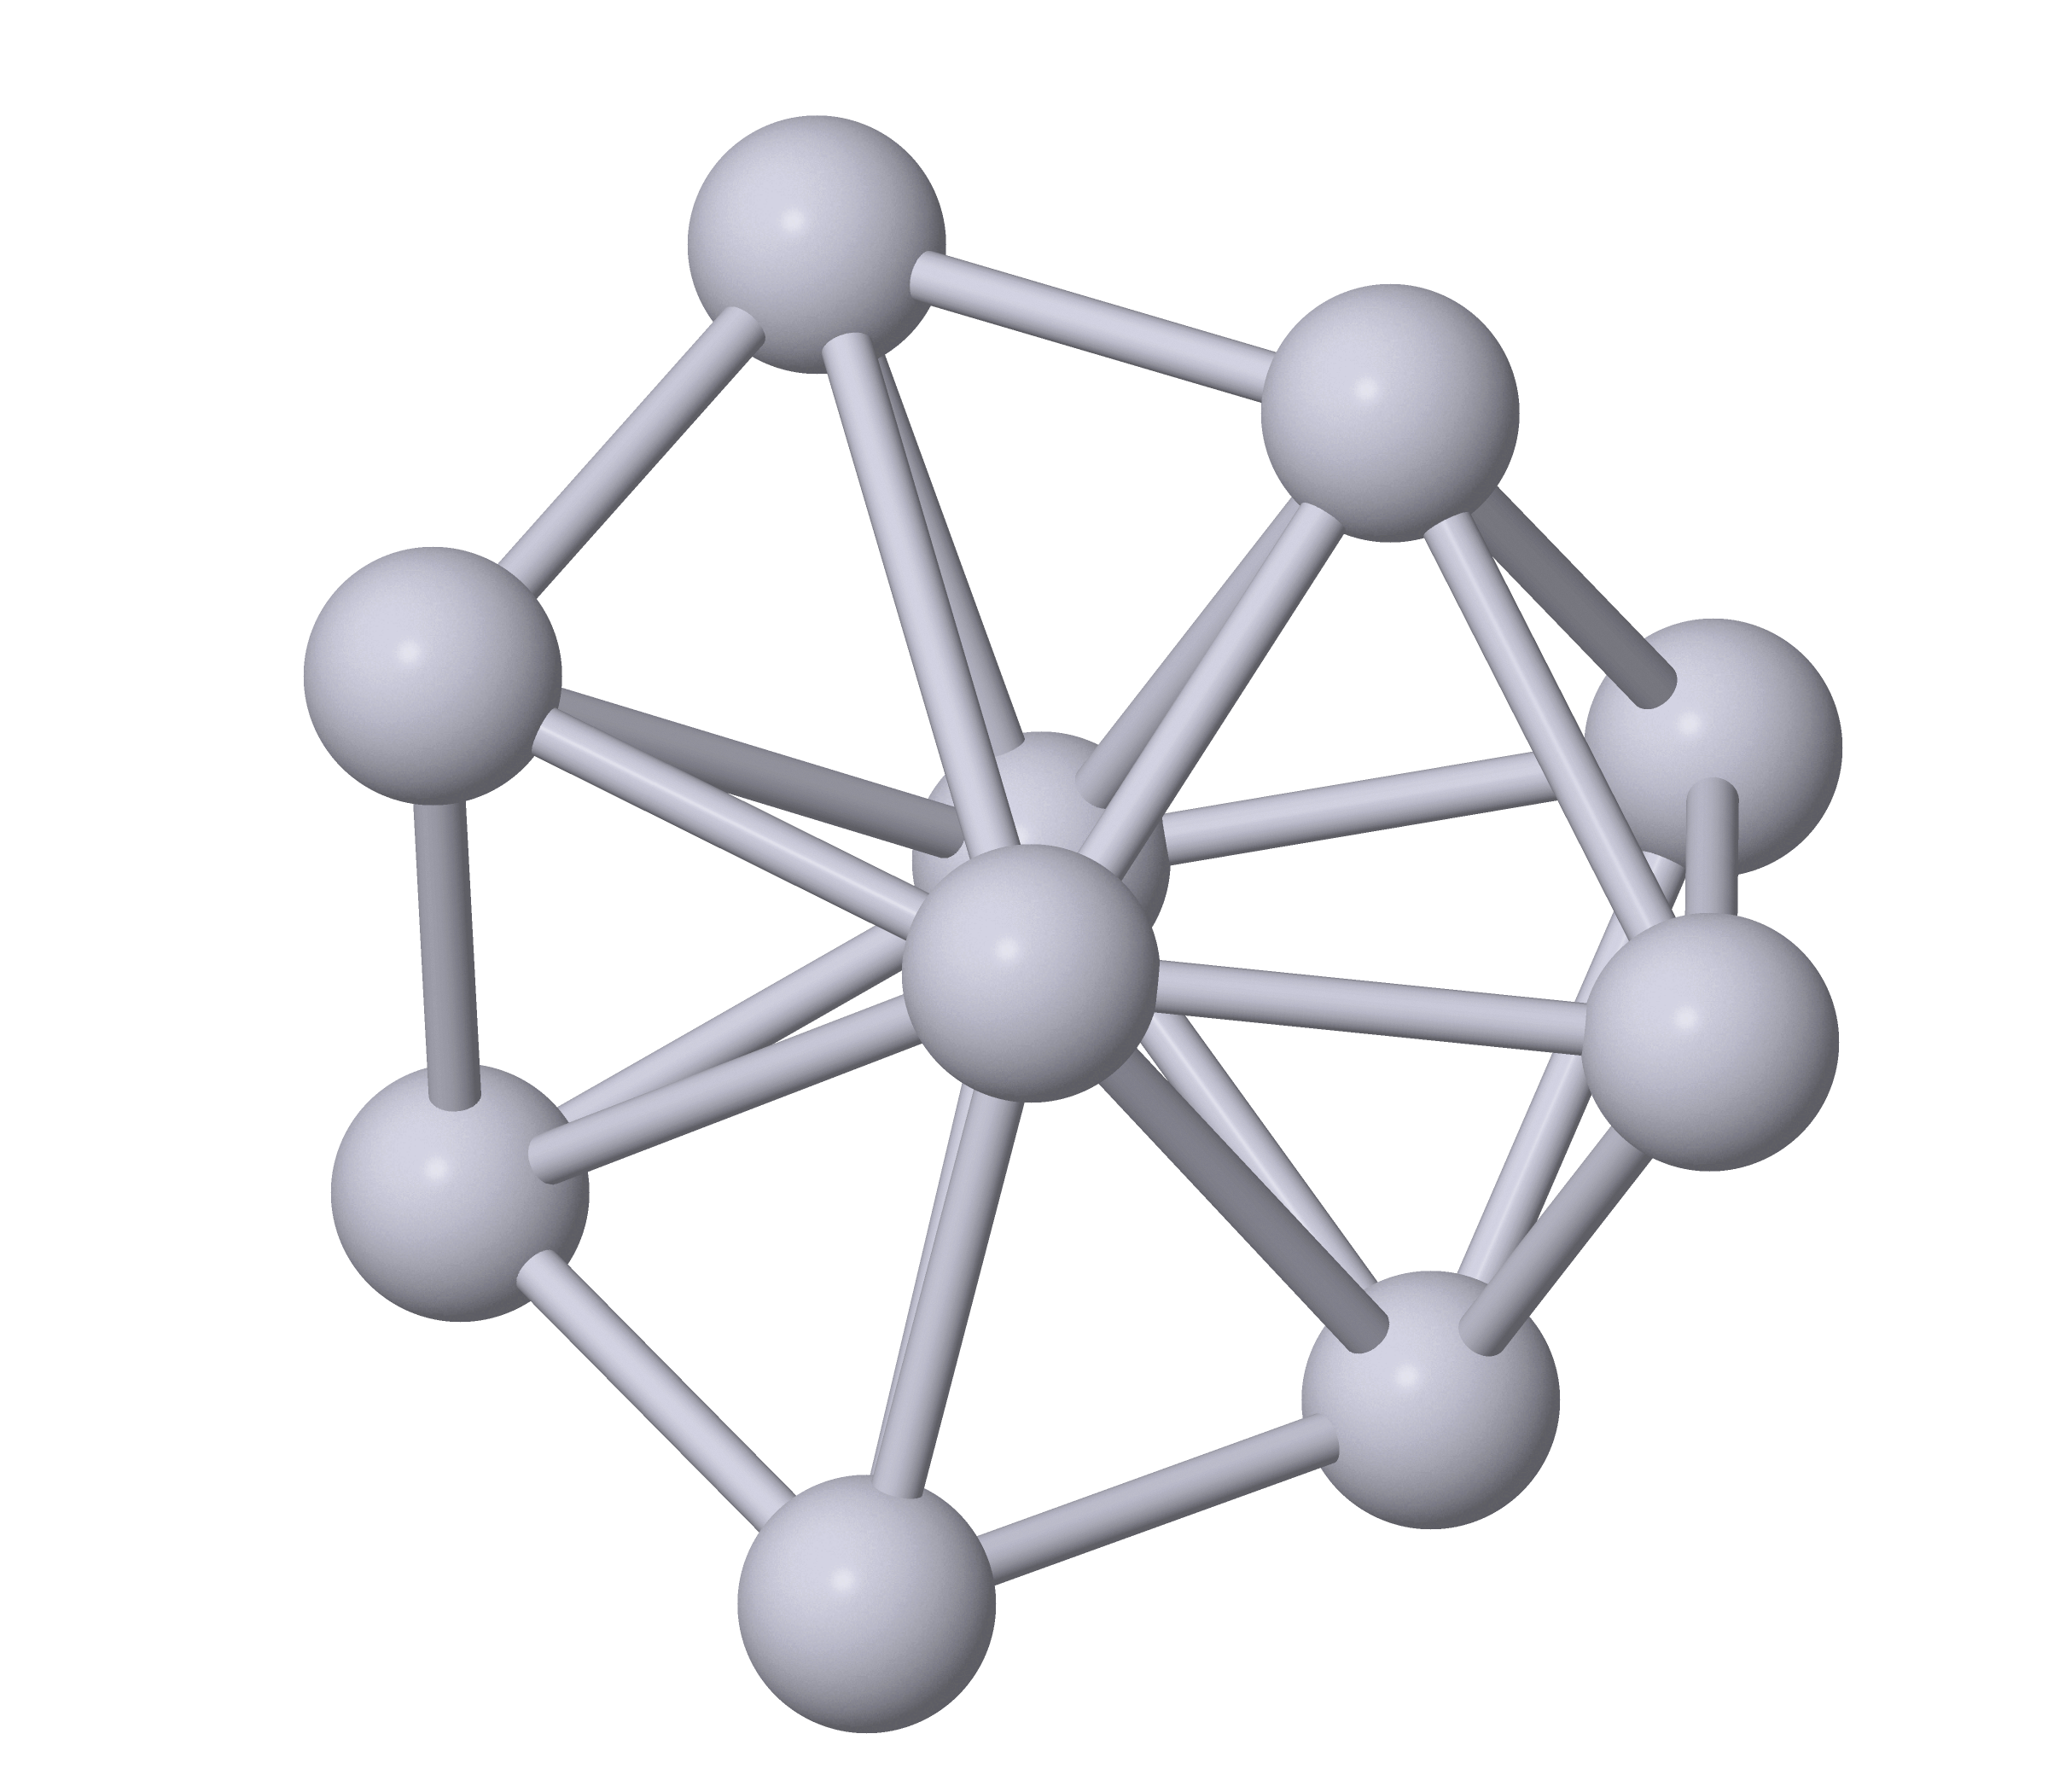
\includegraphics[width=0.62cm]{cl1.png}}; %4
  \node[inner sep=0pt,opacity=0.32] at (4.25,2.32) {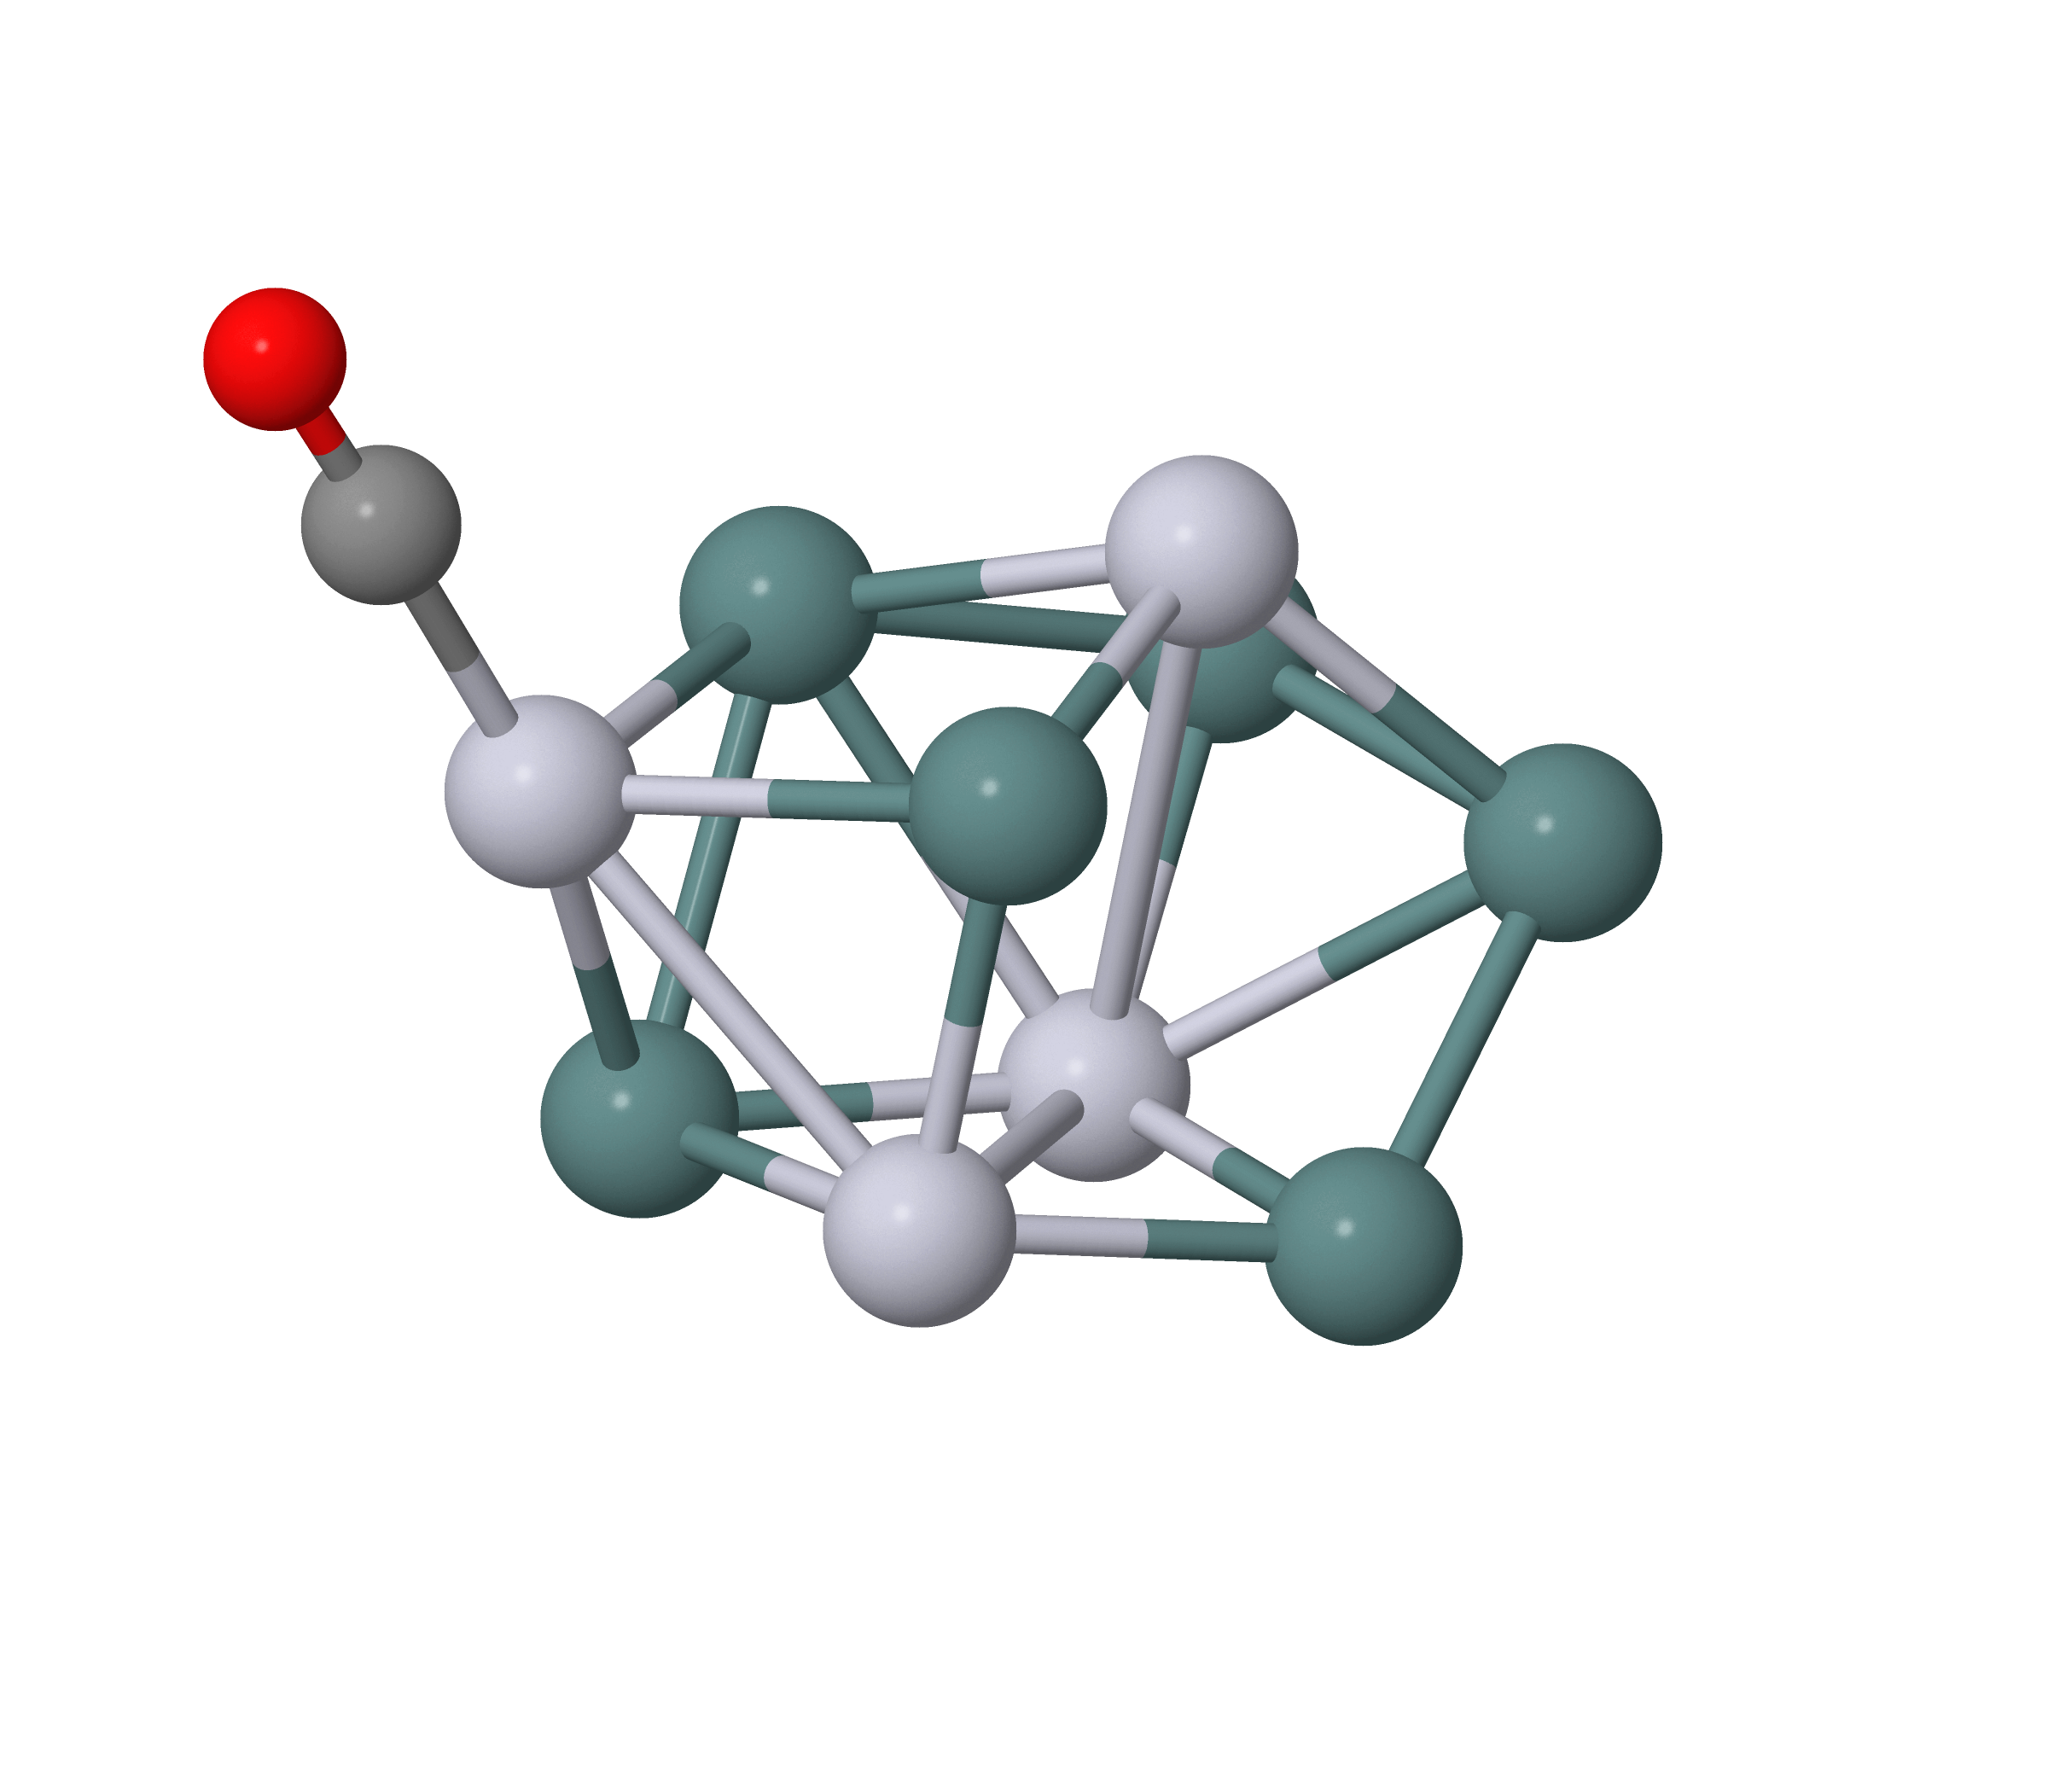
\includegraphics[width=0.70cm]{c6.png}};  %5
  \node[inner sep=0pt,opacity=0.32] at (6.45,2.67)
    {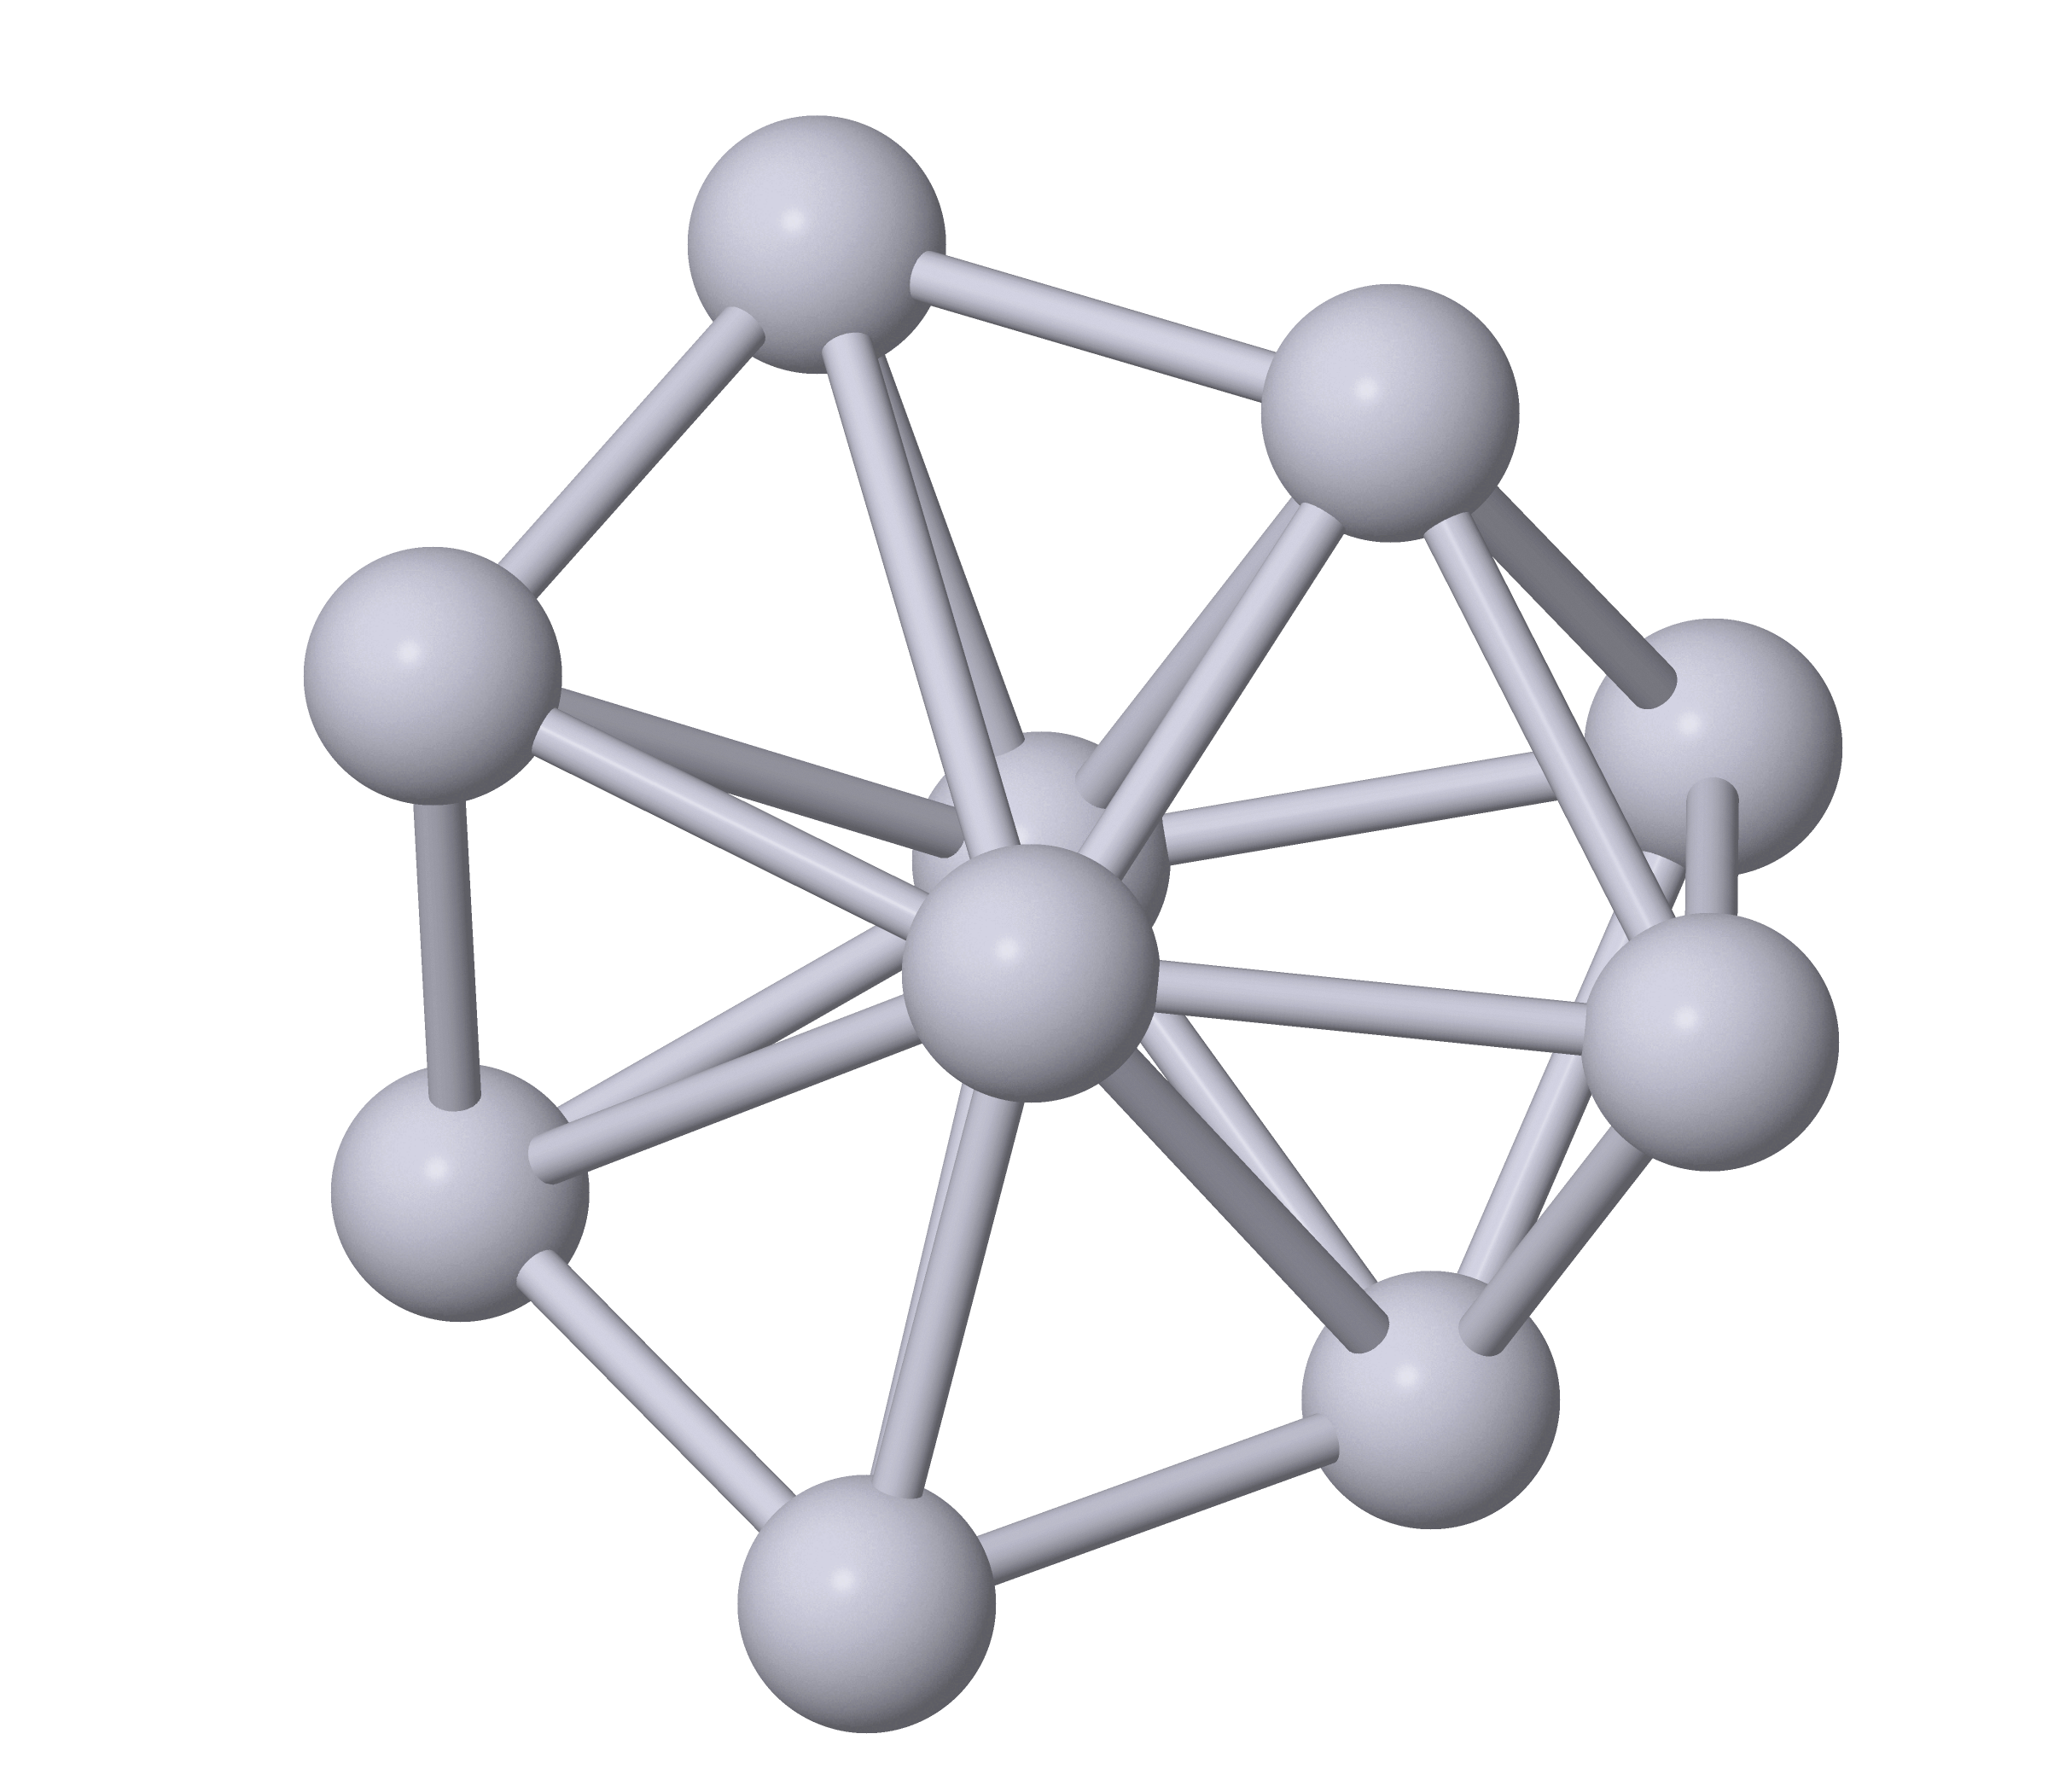
\includegraphics[width=0.58cm,angle=120]{cl1.png}}; %6
  \node[inner sep=0pt,opacity=0.32] at (6.70,0.30) {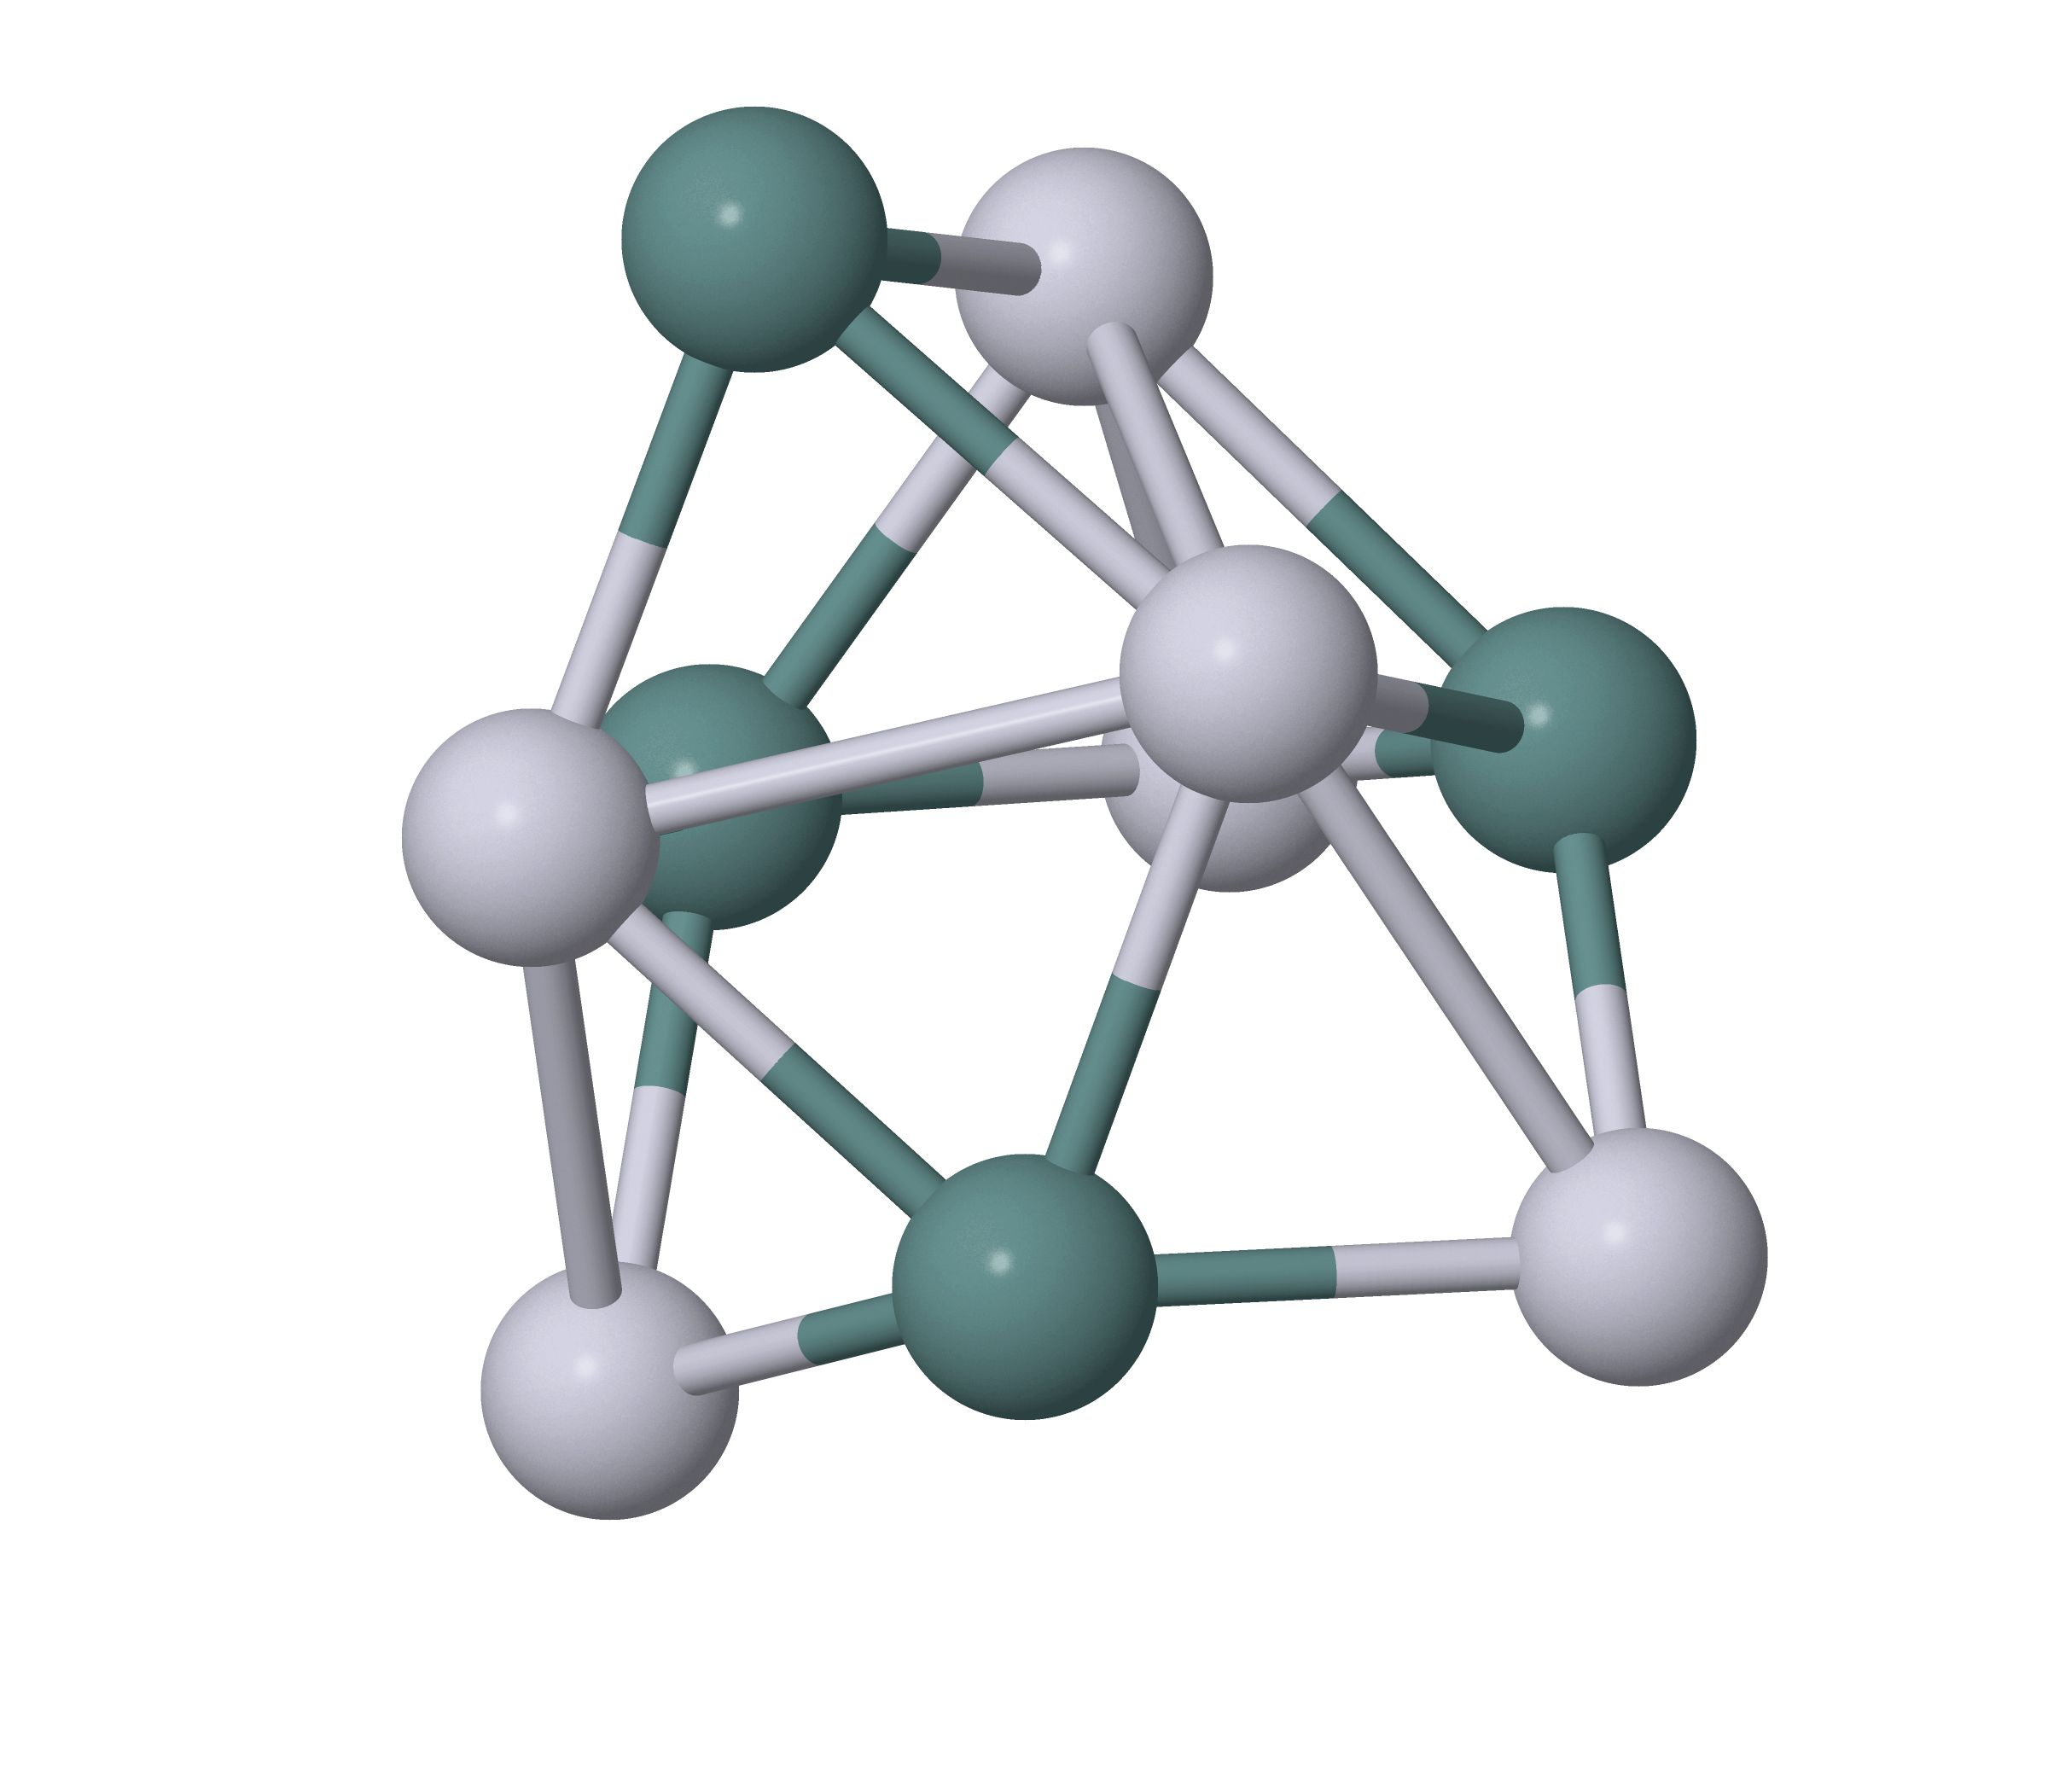
\includegraphics[width=0.58cm]{c2.png}};  %7
  \node[inner sep=0pt,opacity=0.30] at (7.16,1.58) {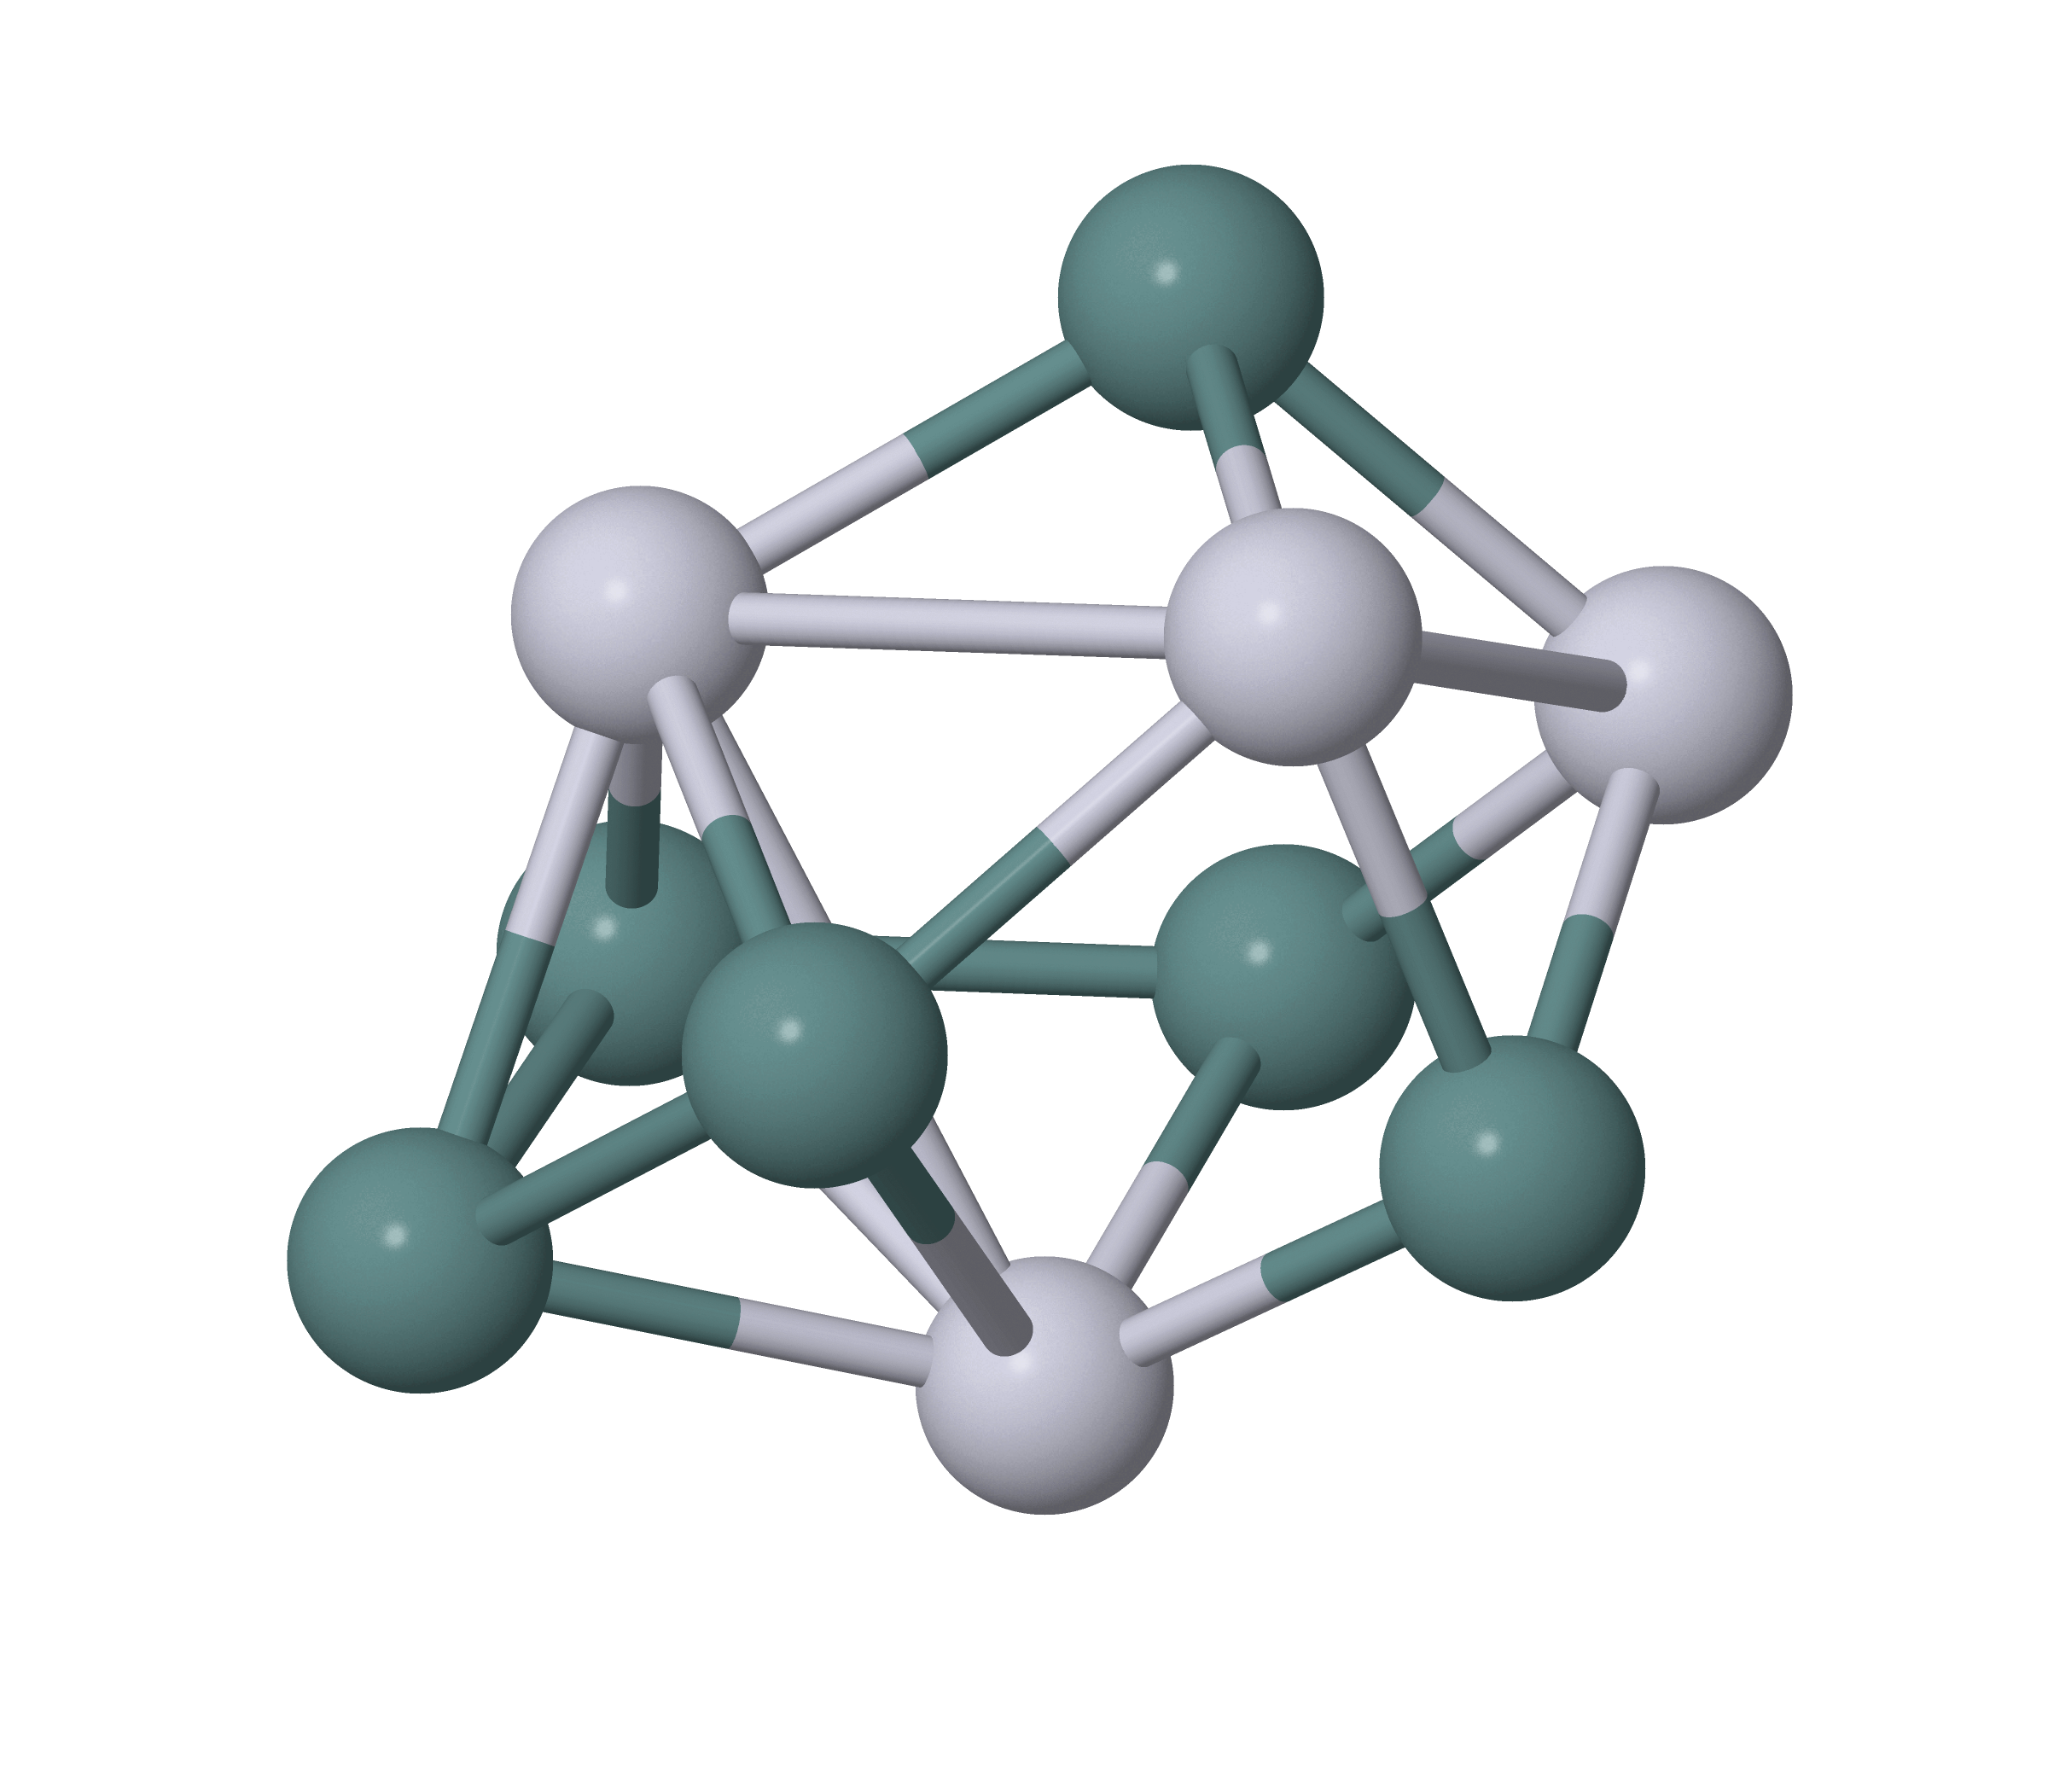
\includegraphics[width=0.72cm,angle=45]{c3.png}};
  \node[inner sep=0pt,opacity=0.3] at (7.35,0.52) {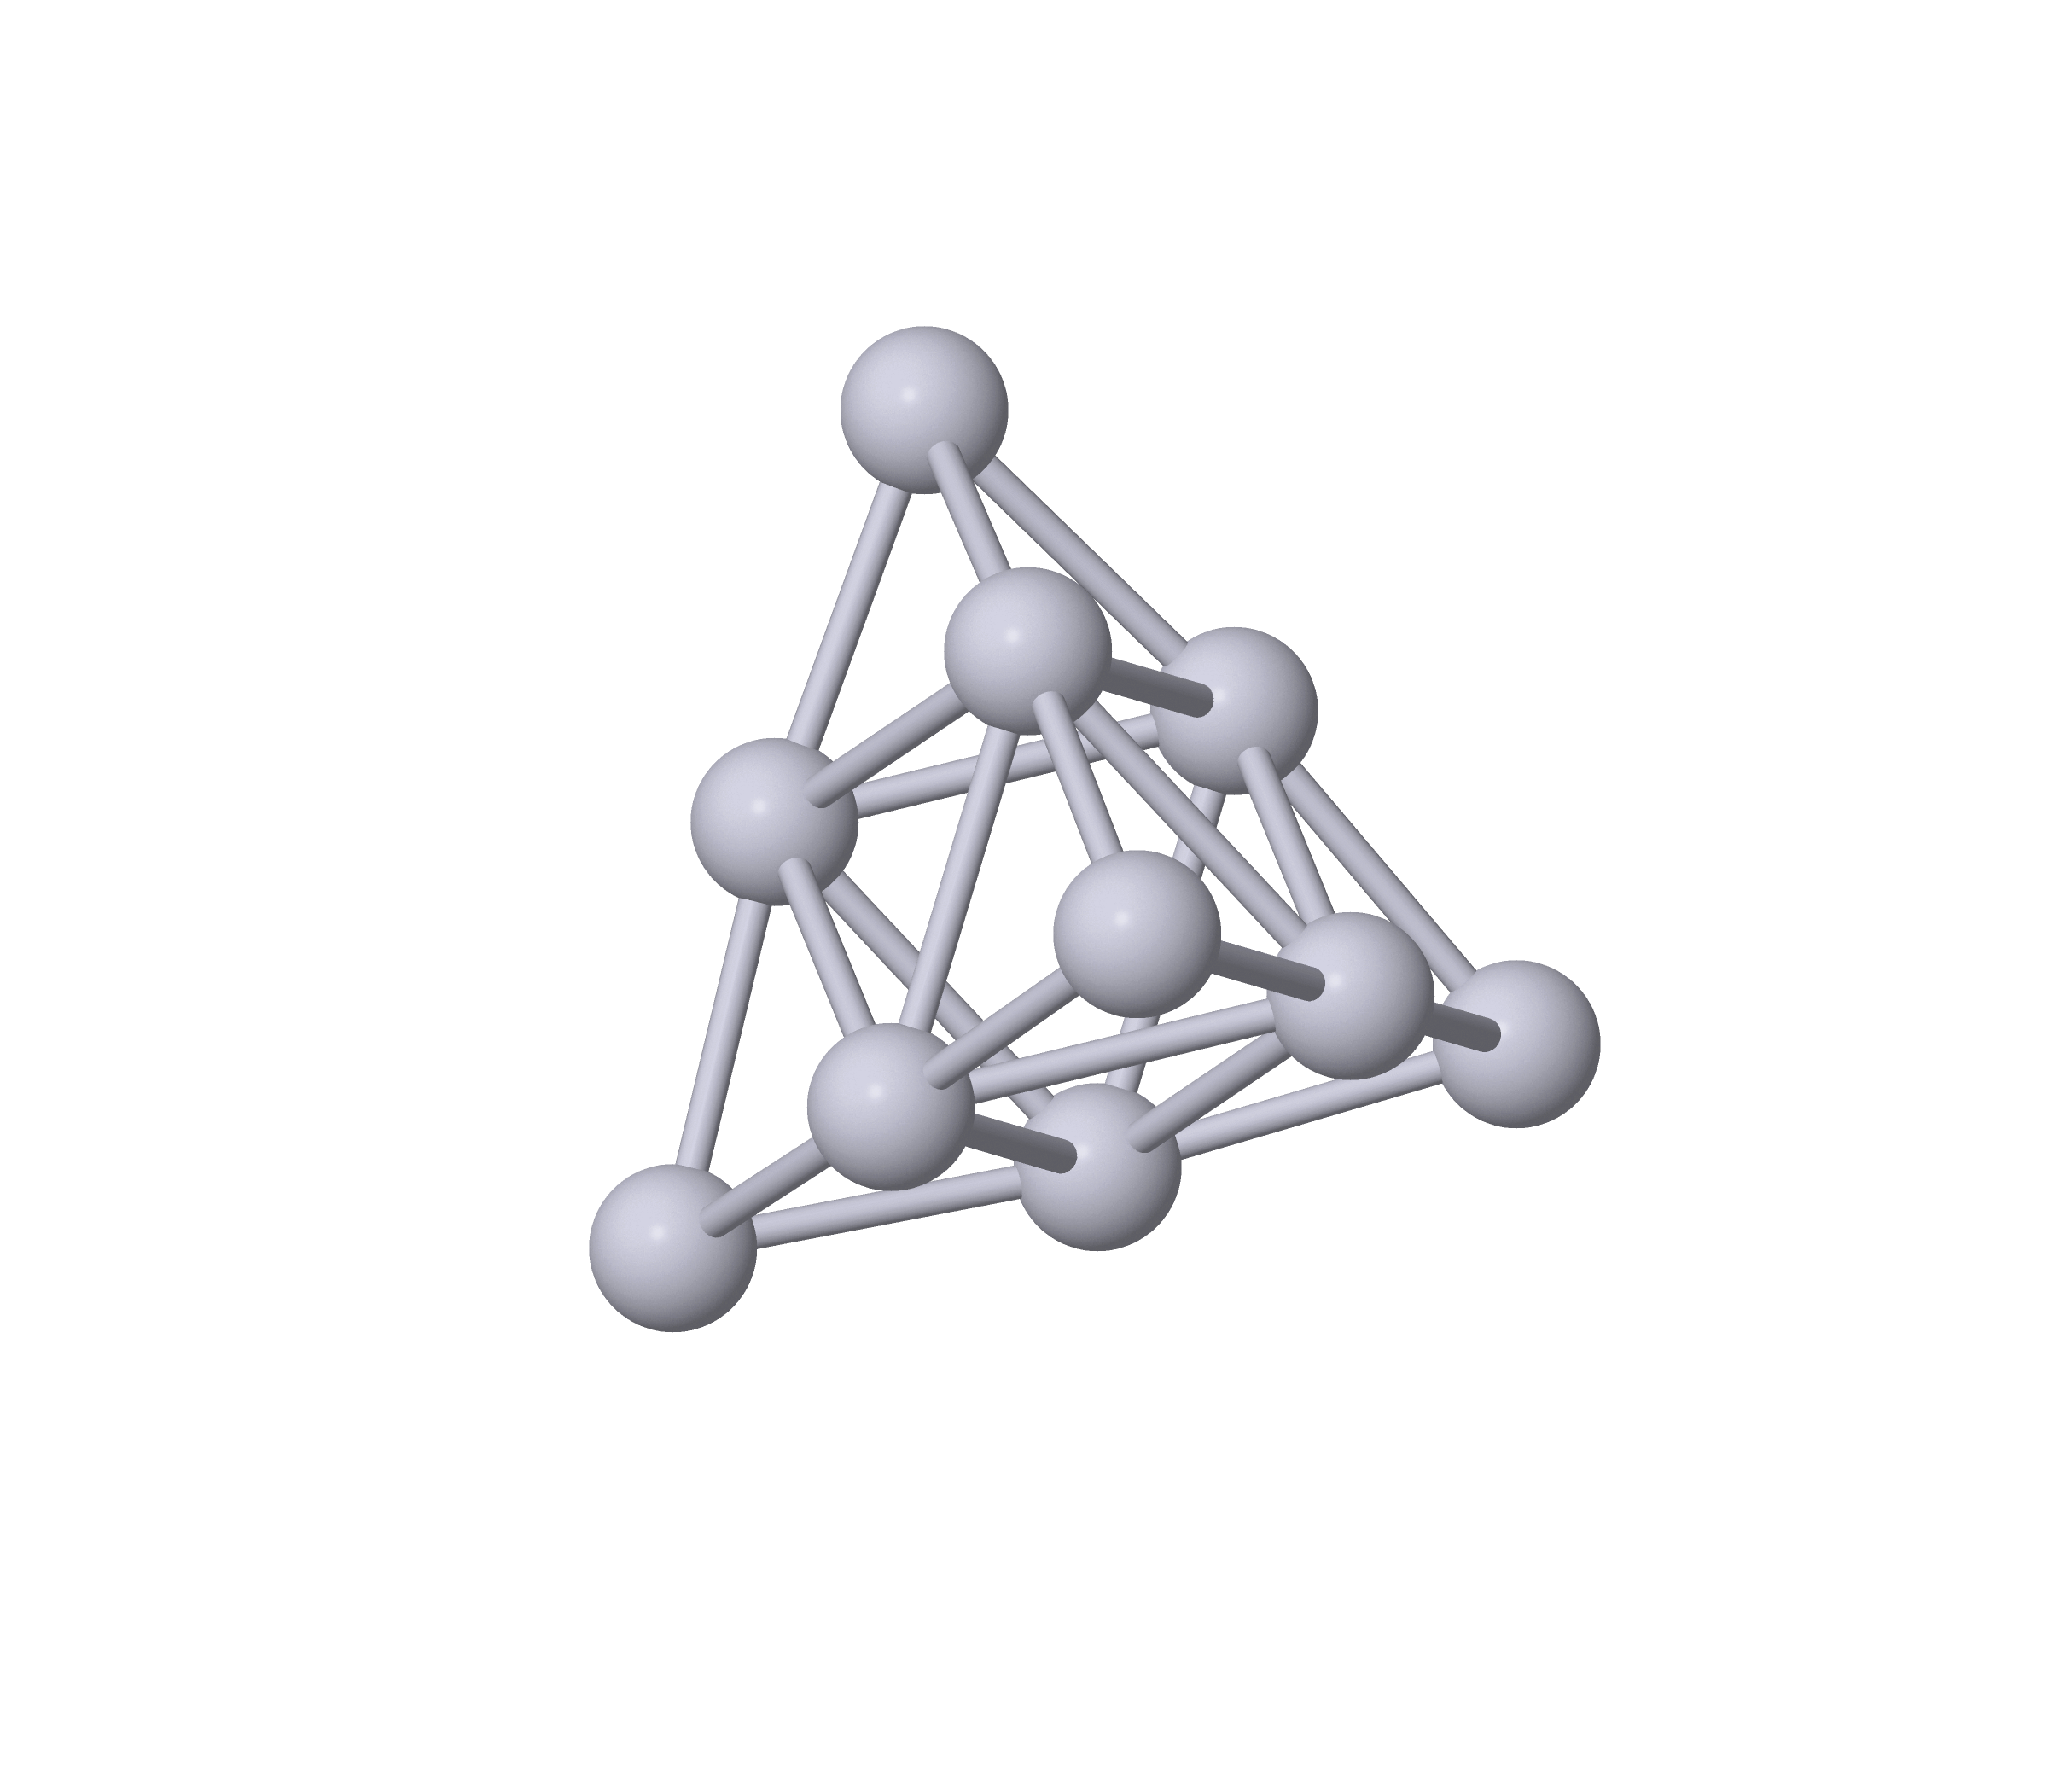
\includegraphics[width=0.80cm]{c5.png}};
  % New structures placed at the approximate positions marked for review.
  \node[inner sep=0pt,opacity=0.32] at (1.58,2.68) {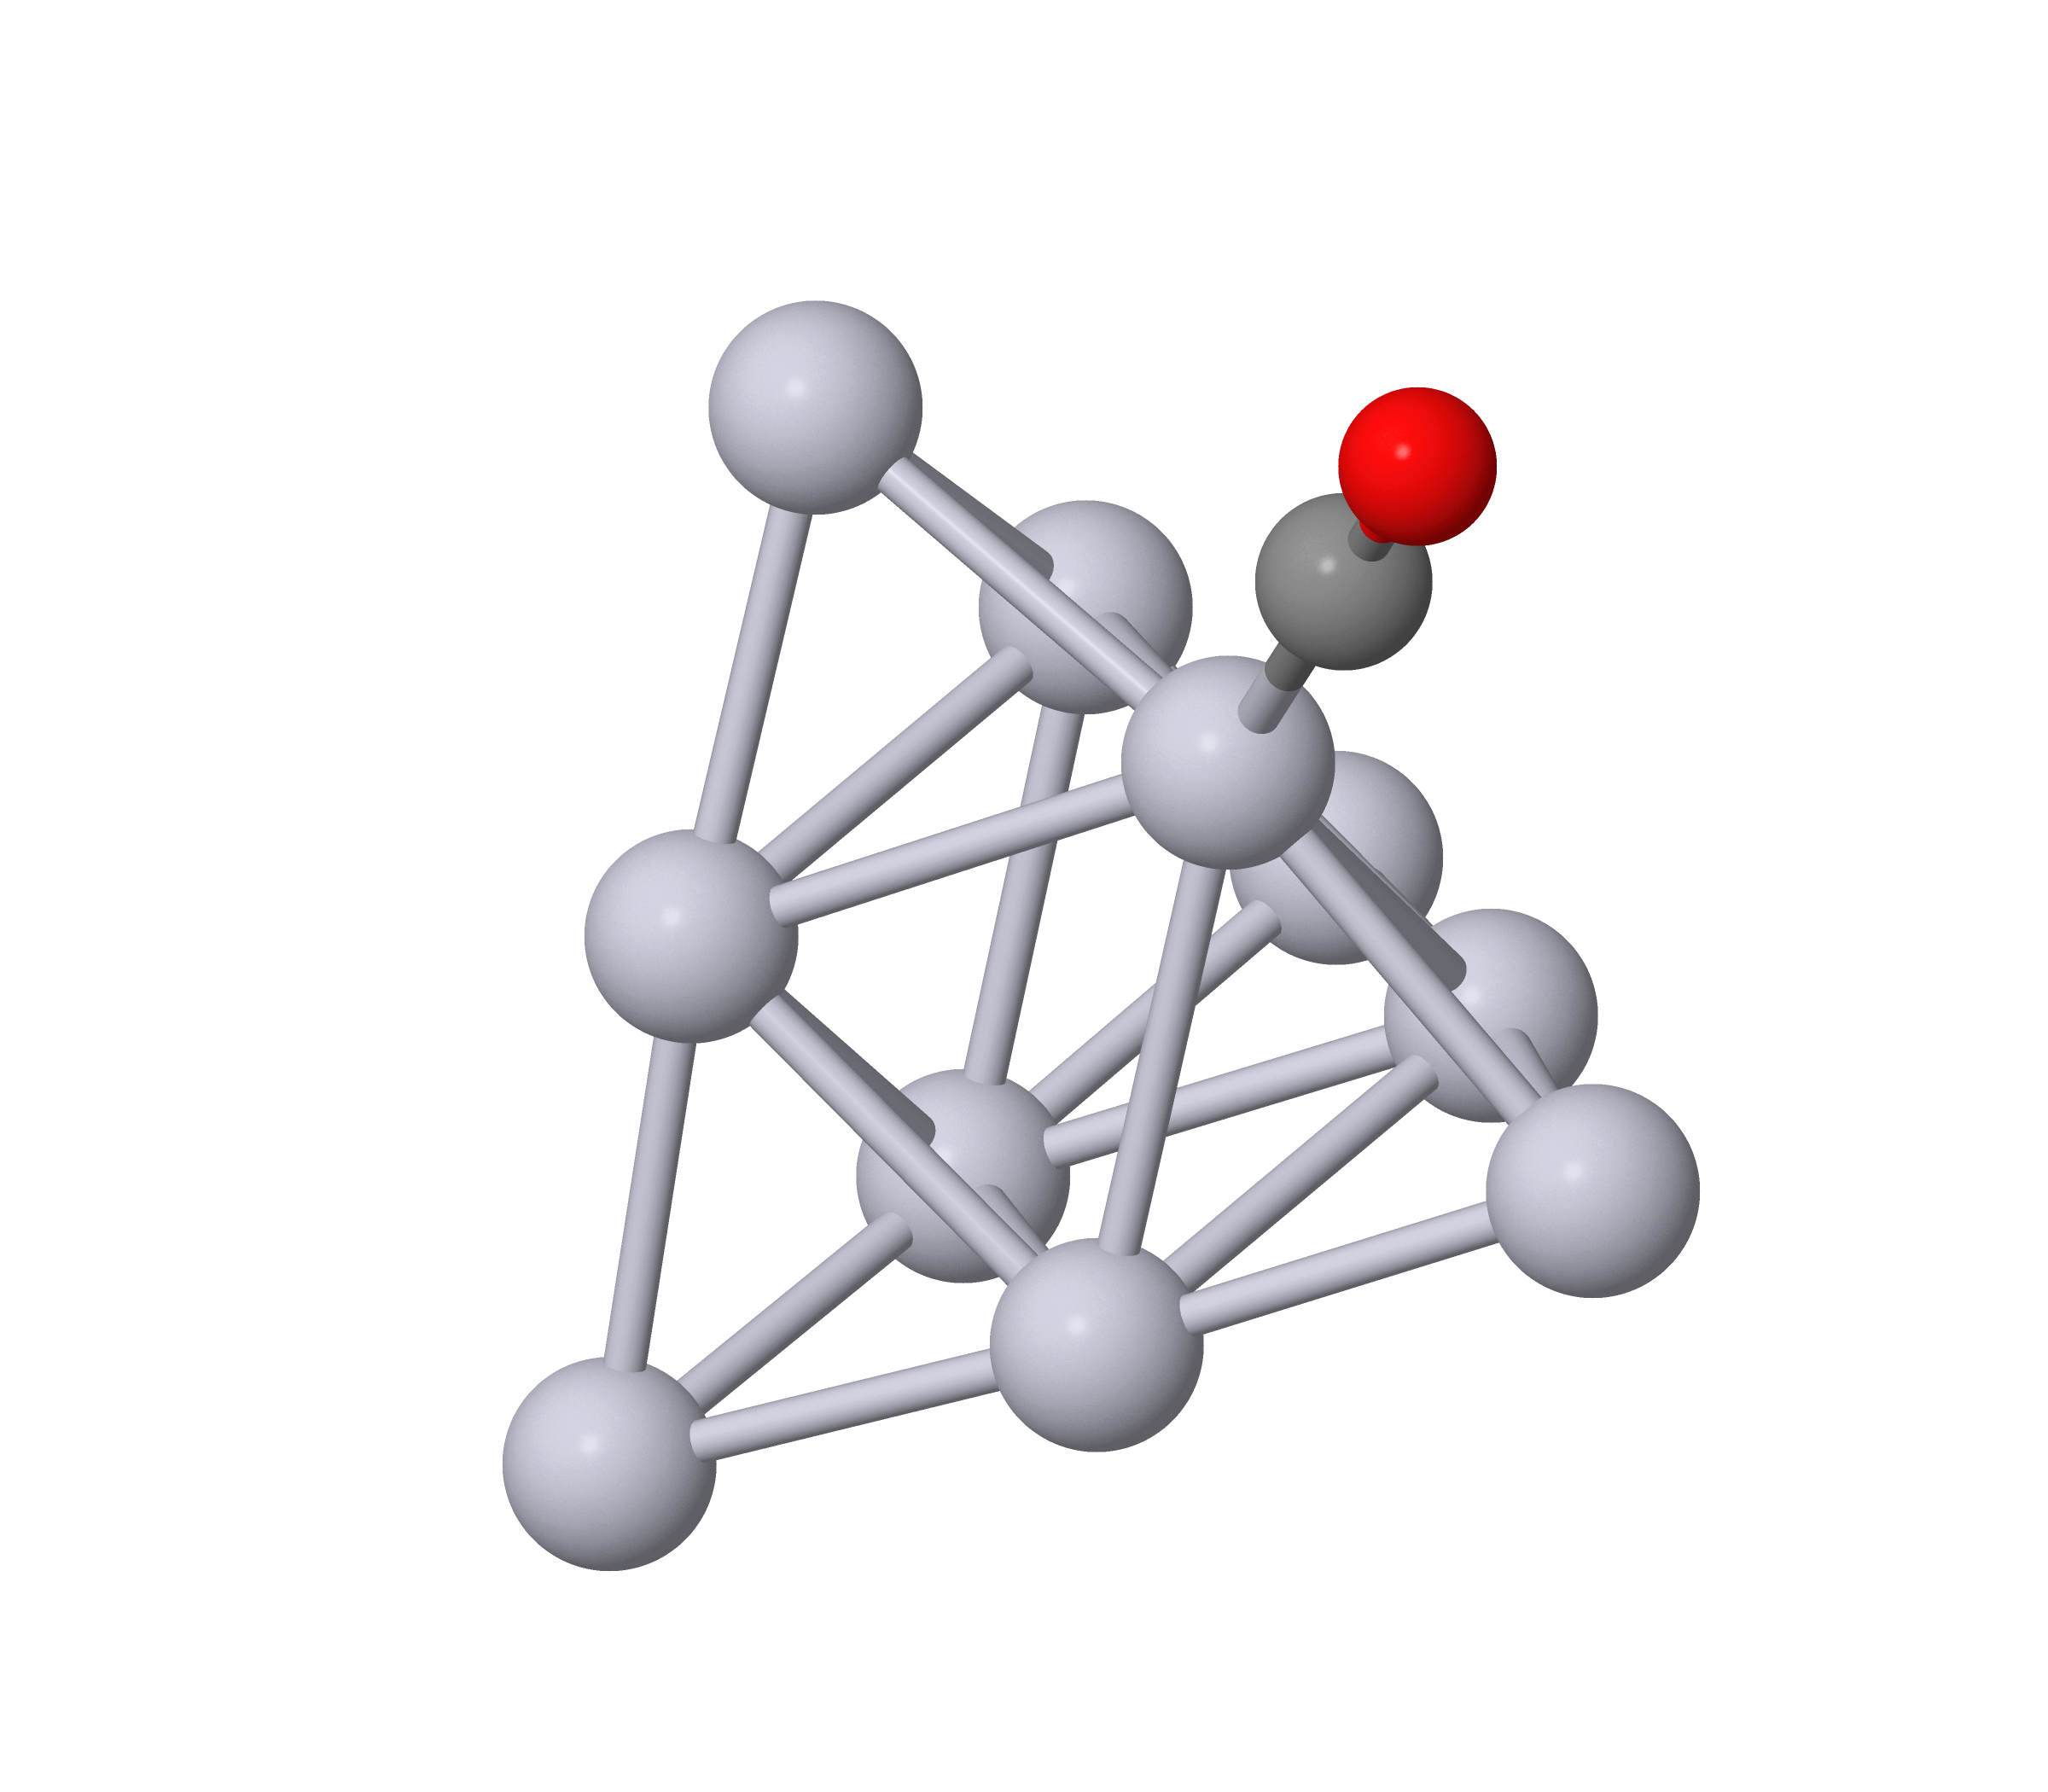
\includegraphics[width=0.68cm]{cA.png}};
  \node[inner sep=0pt,opacity=0.32] at (3.24,1.18) {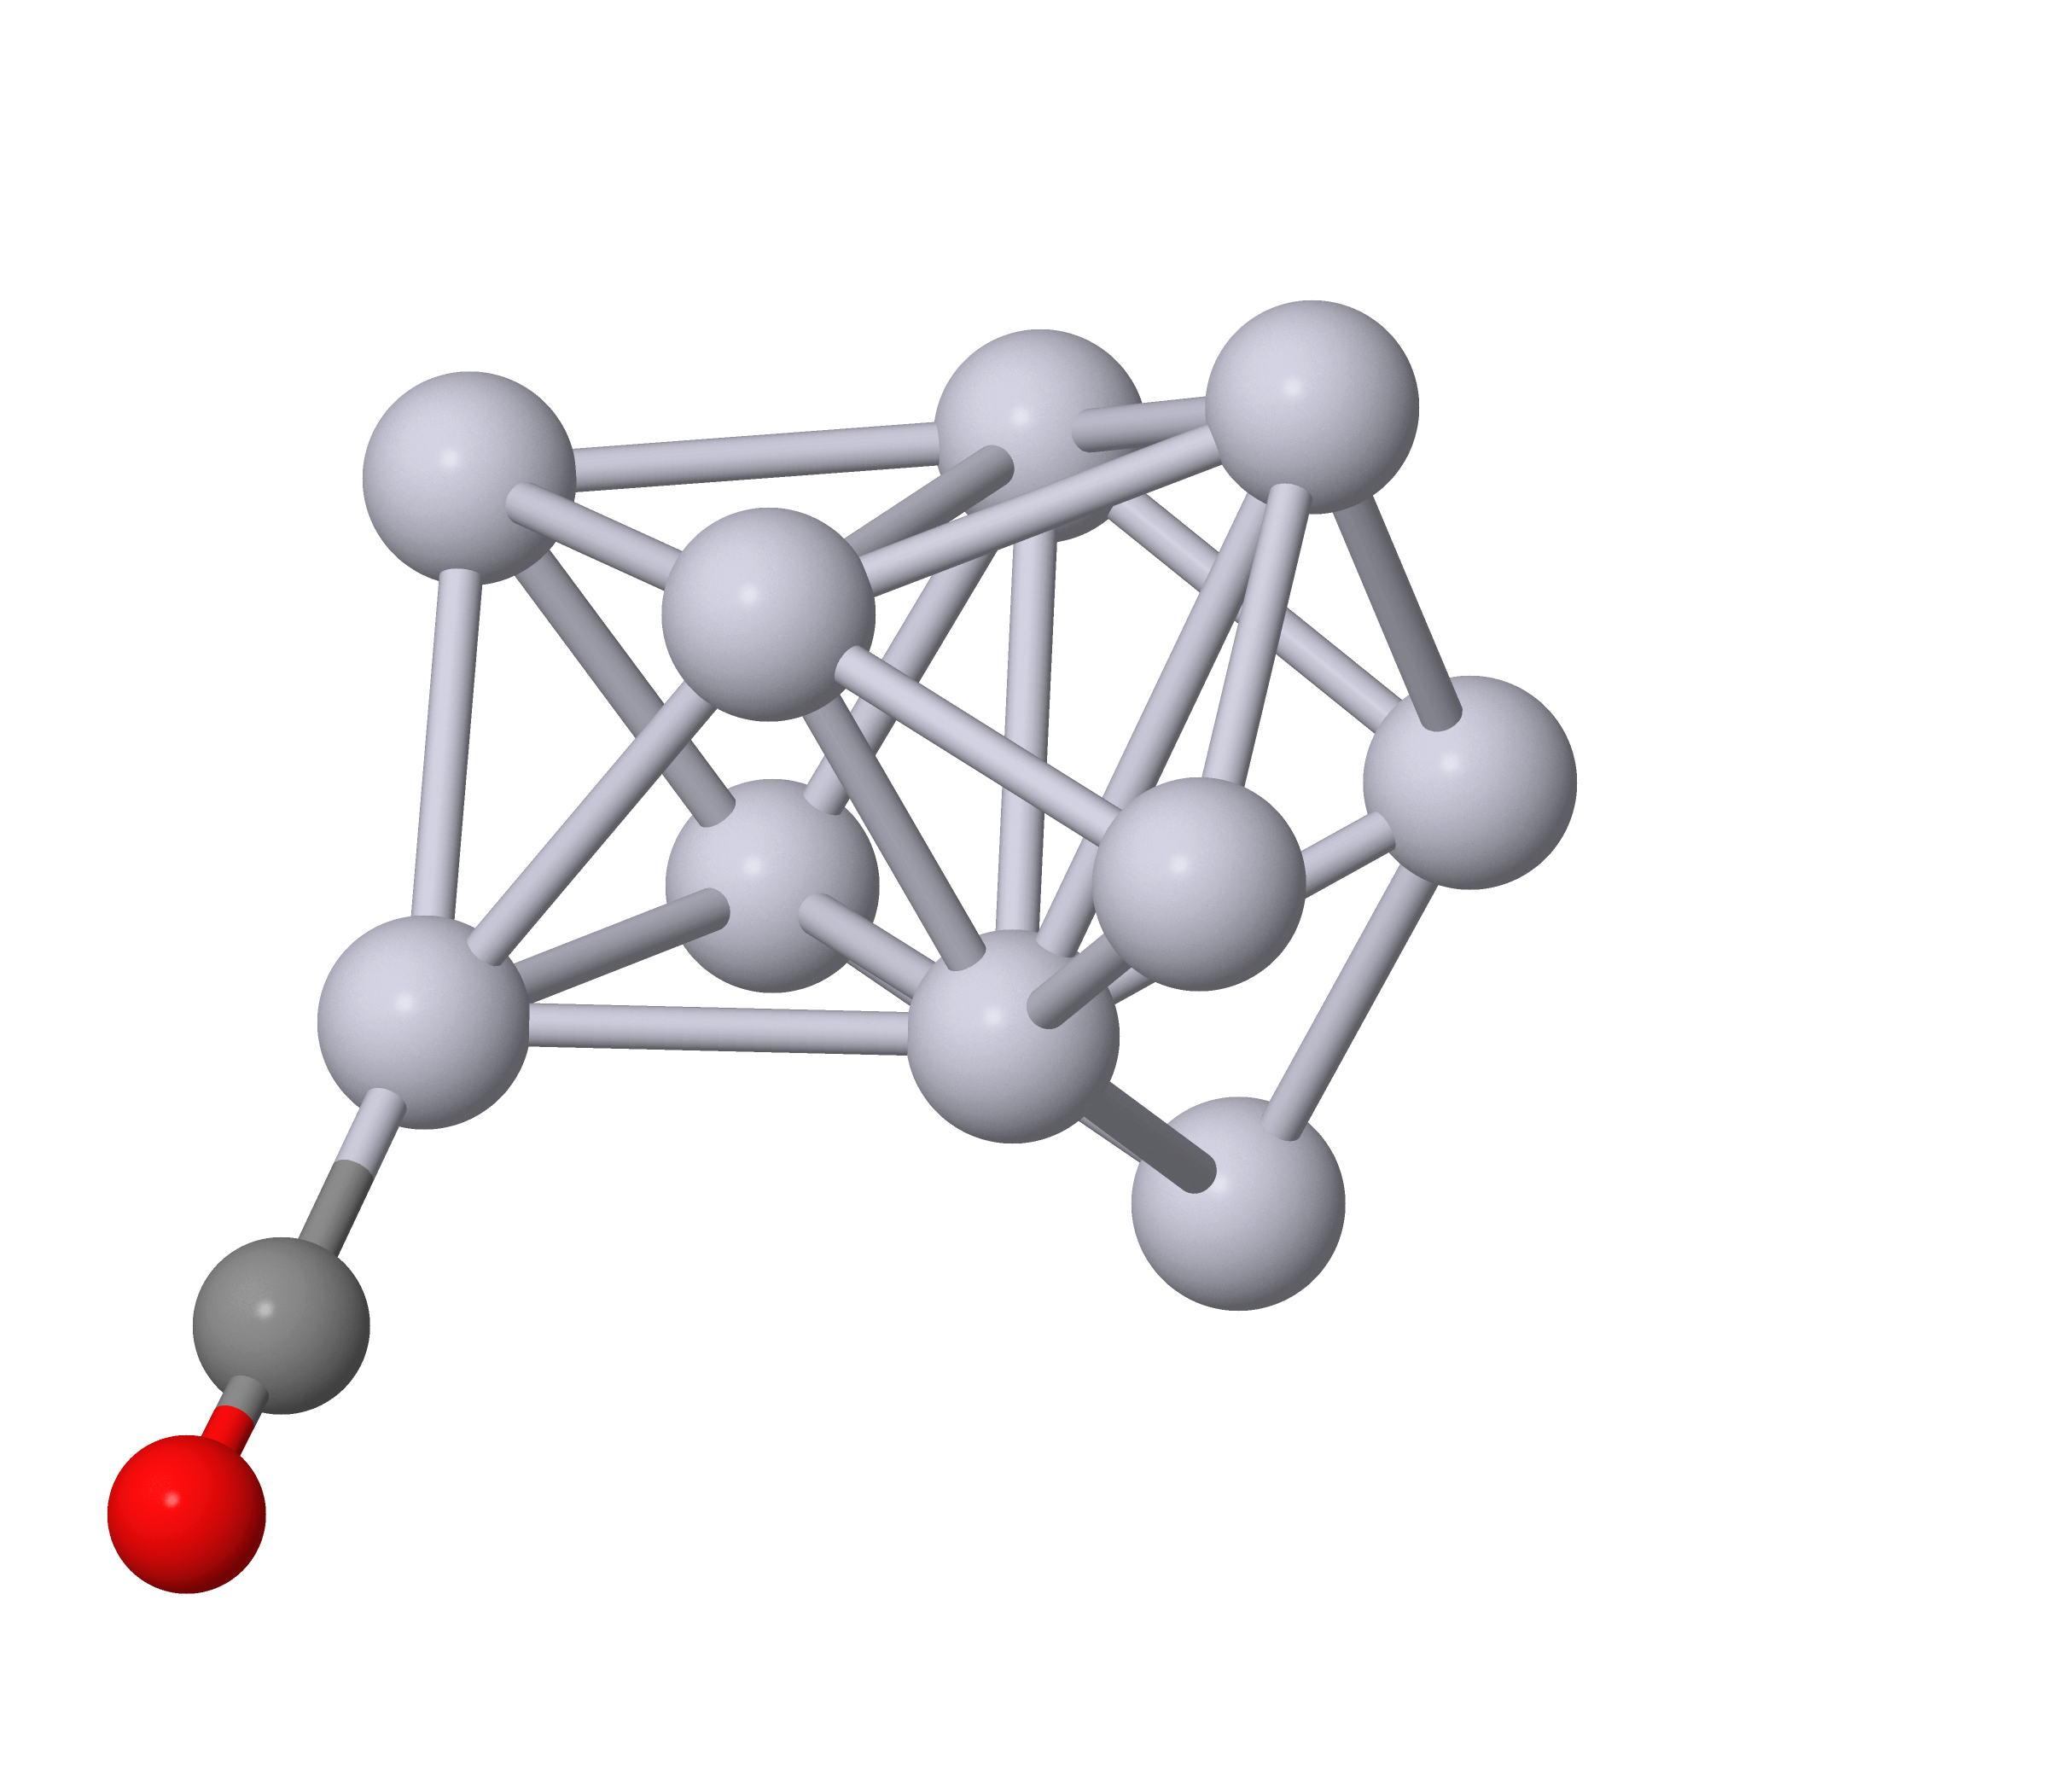
\includegraphics[width=0.68cm]{cB.png}};
  \node[inner sep=0pt,opacity=0.32] at (2.47,0.43) {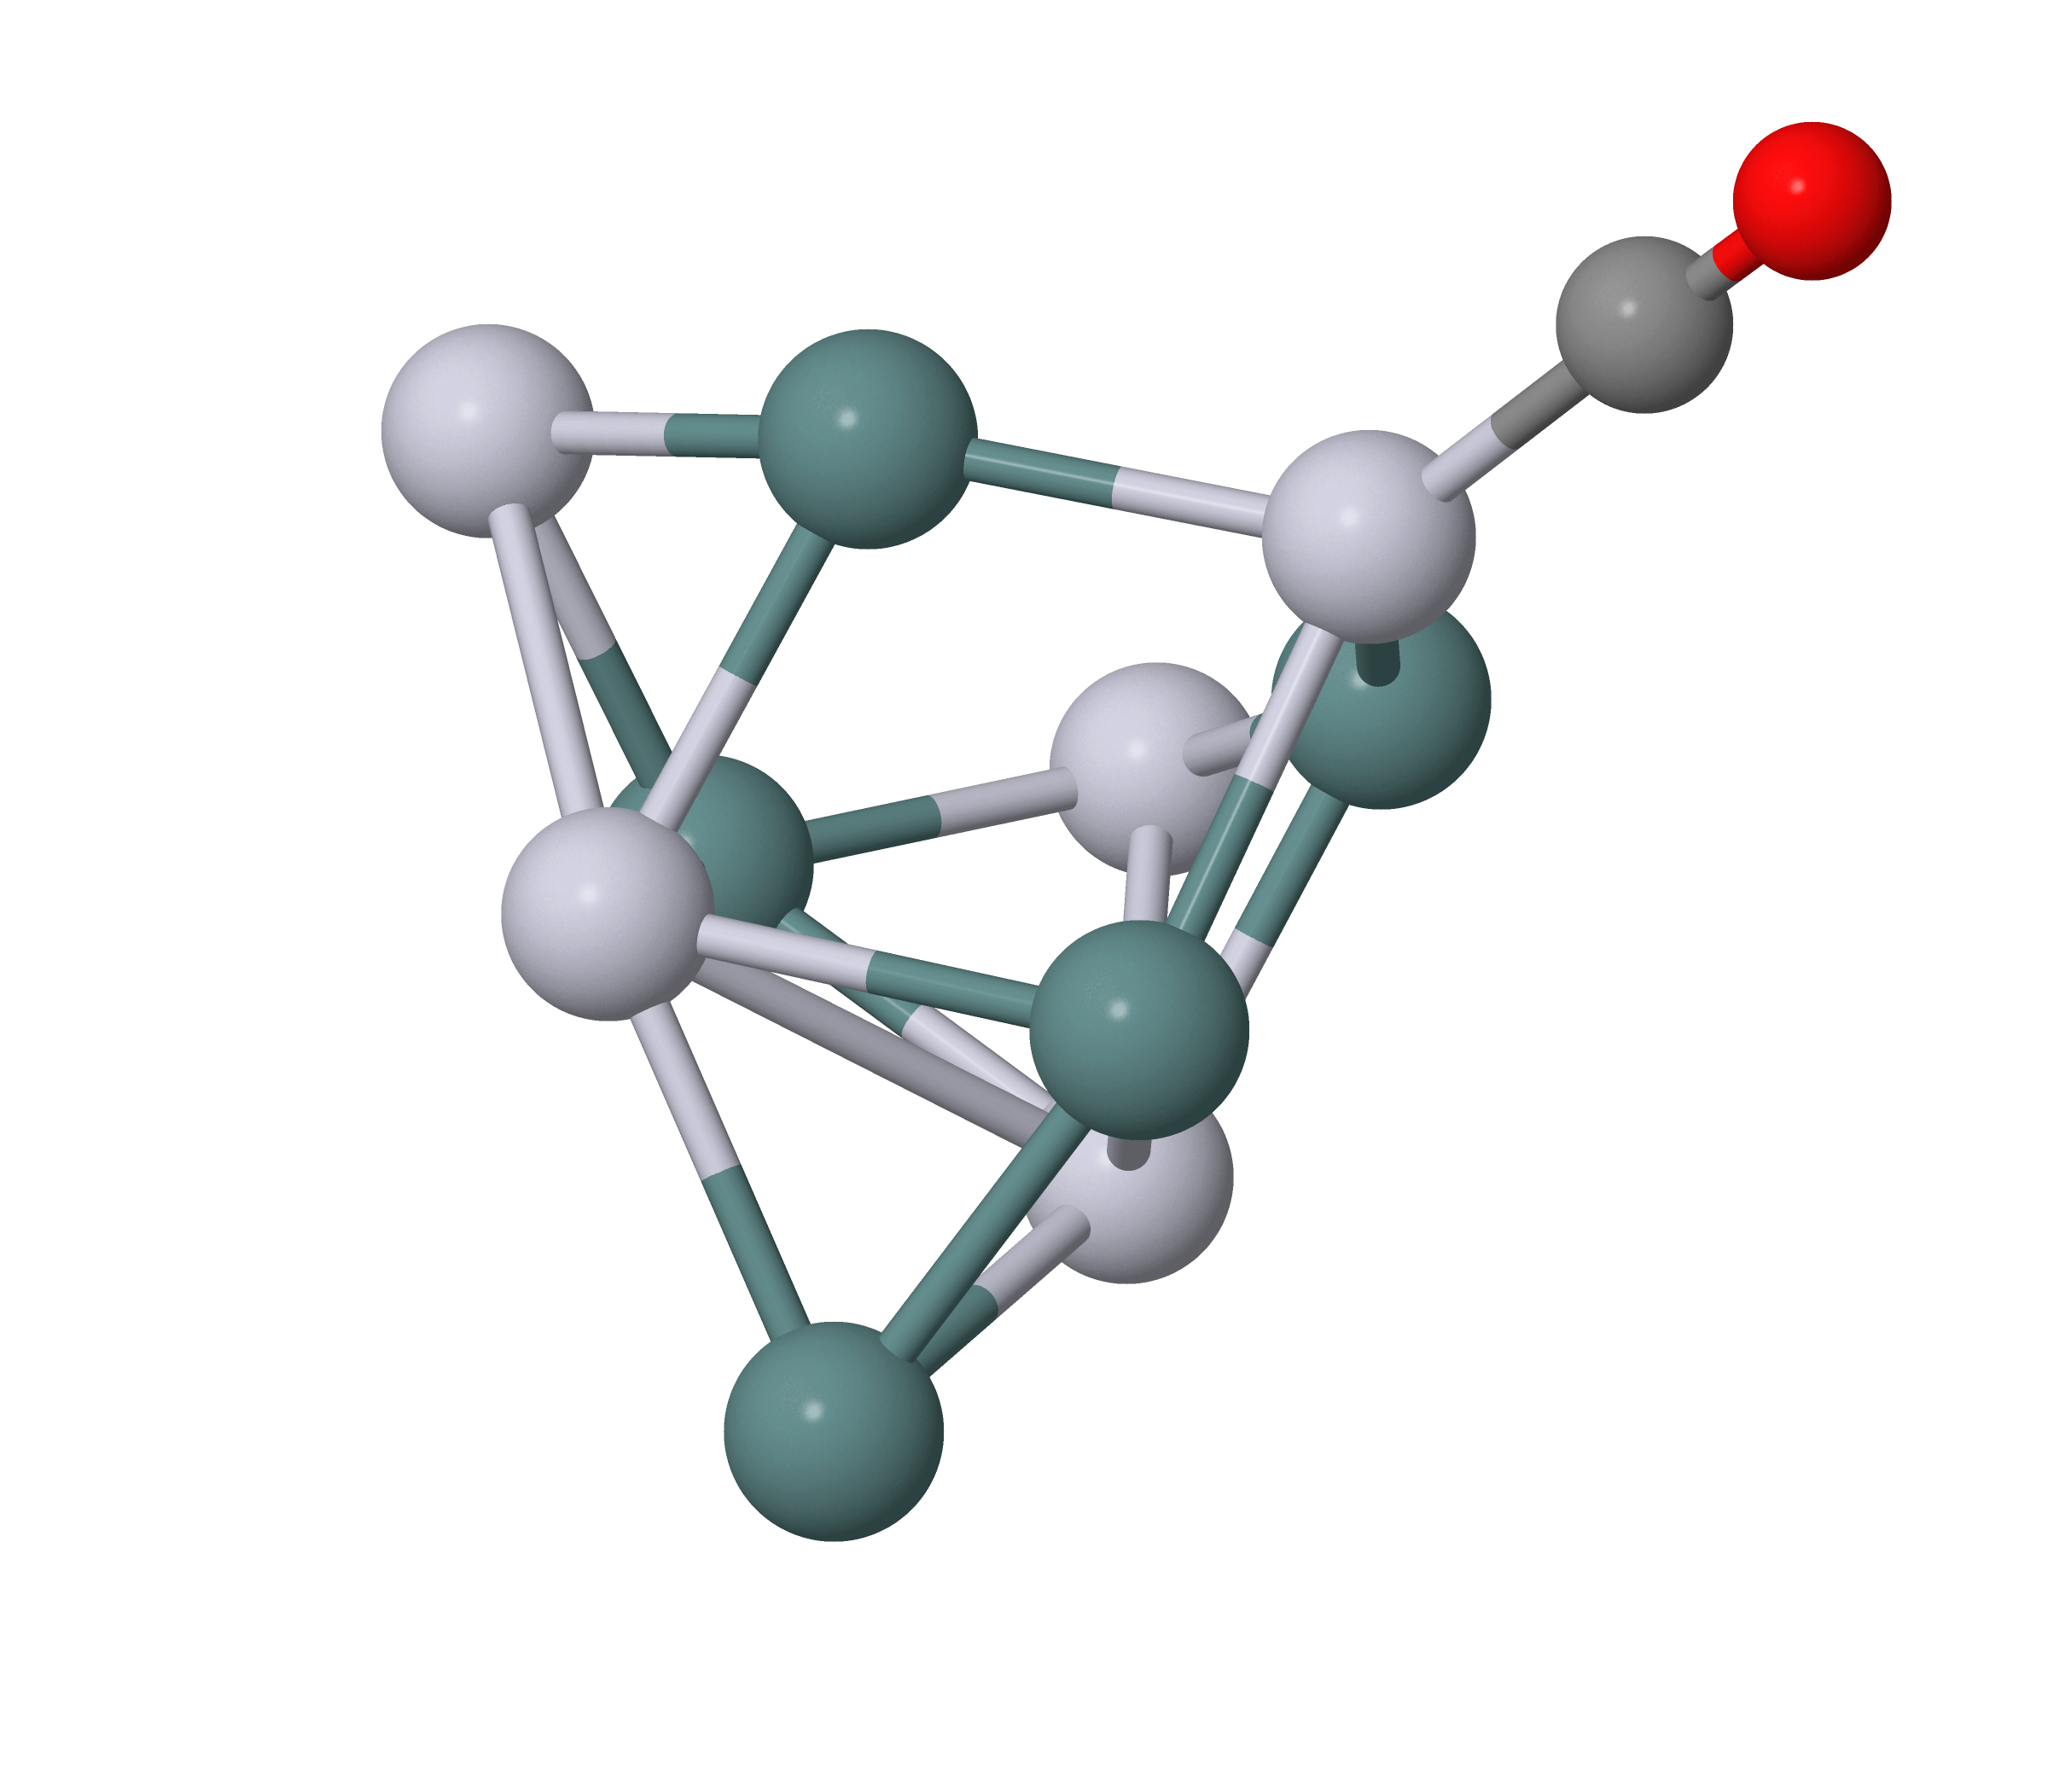
\includegraphics[width=0.68cm]{cD.png}};

  \node[inner sep=0pt] at (1.02,1.63) {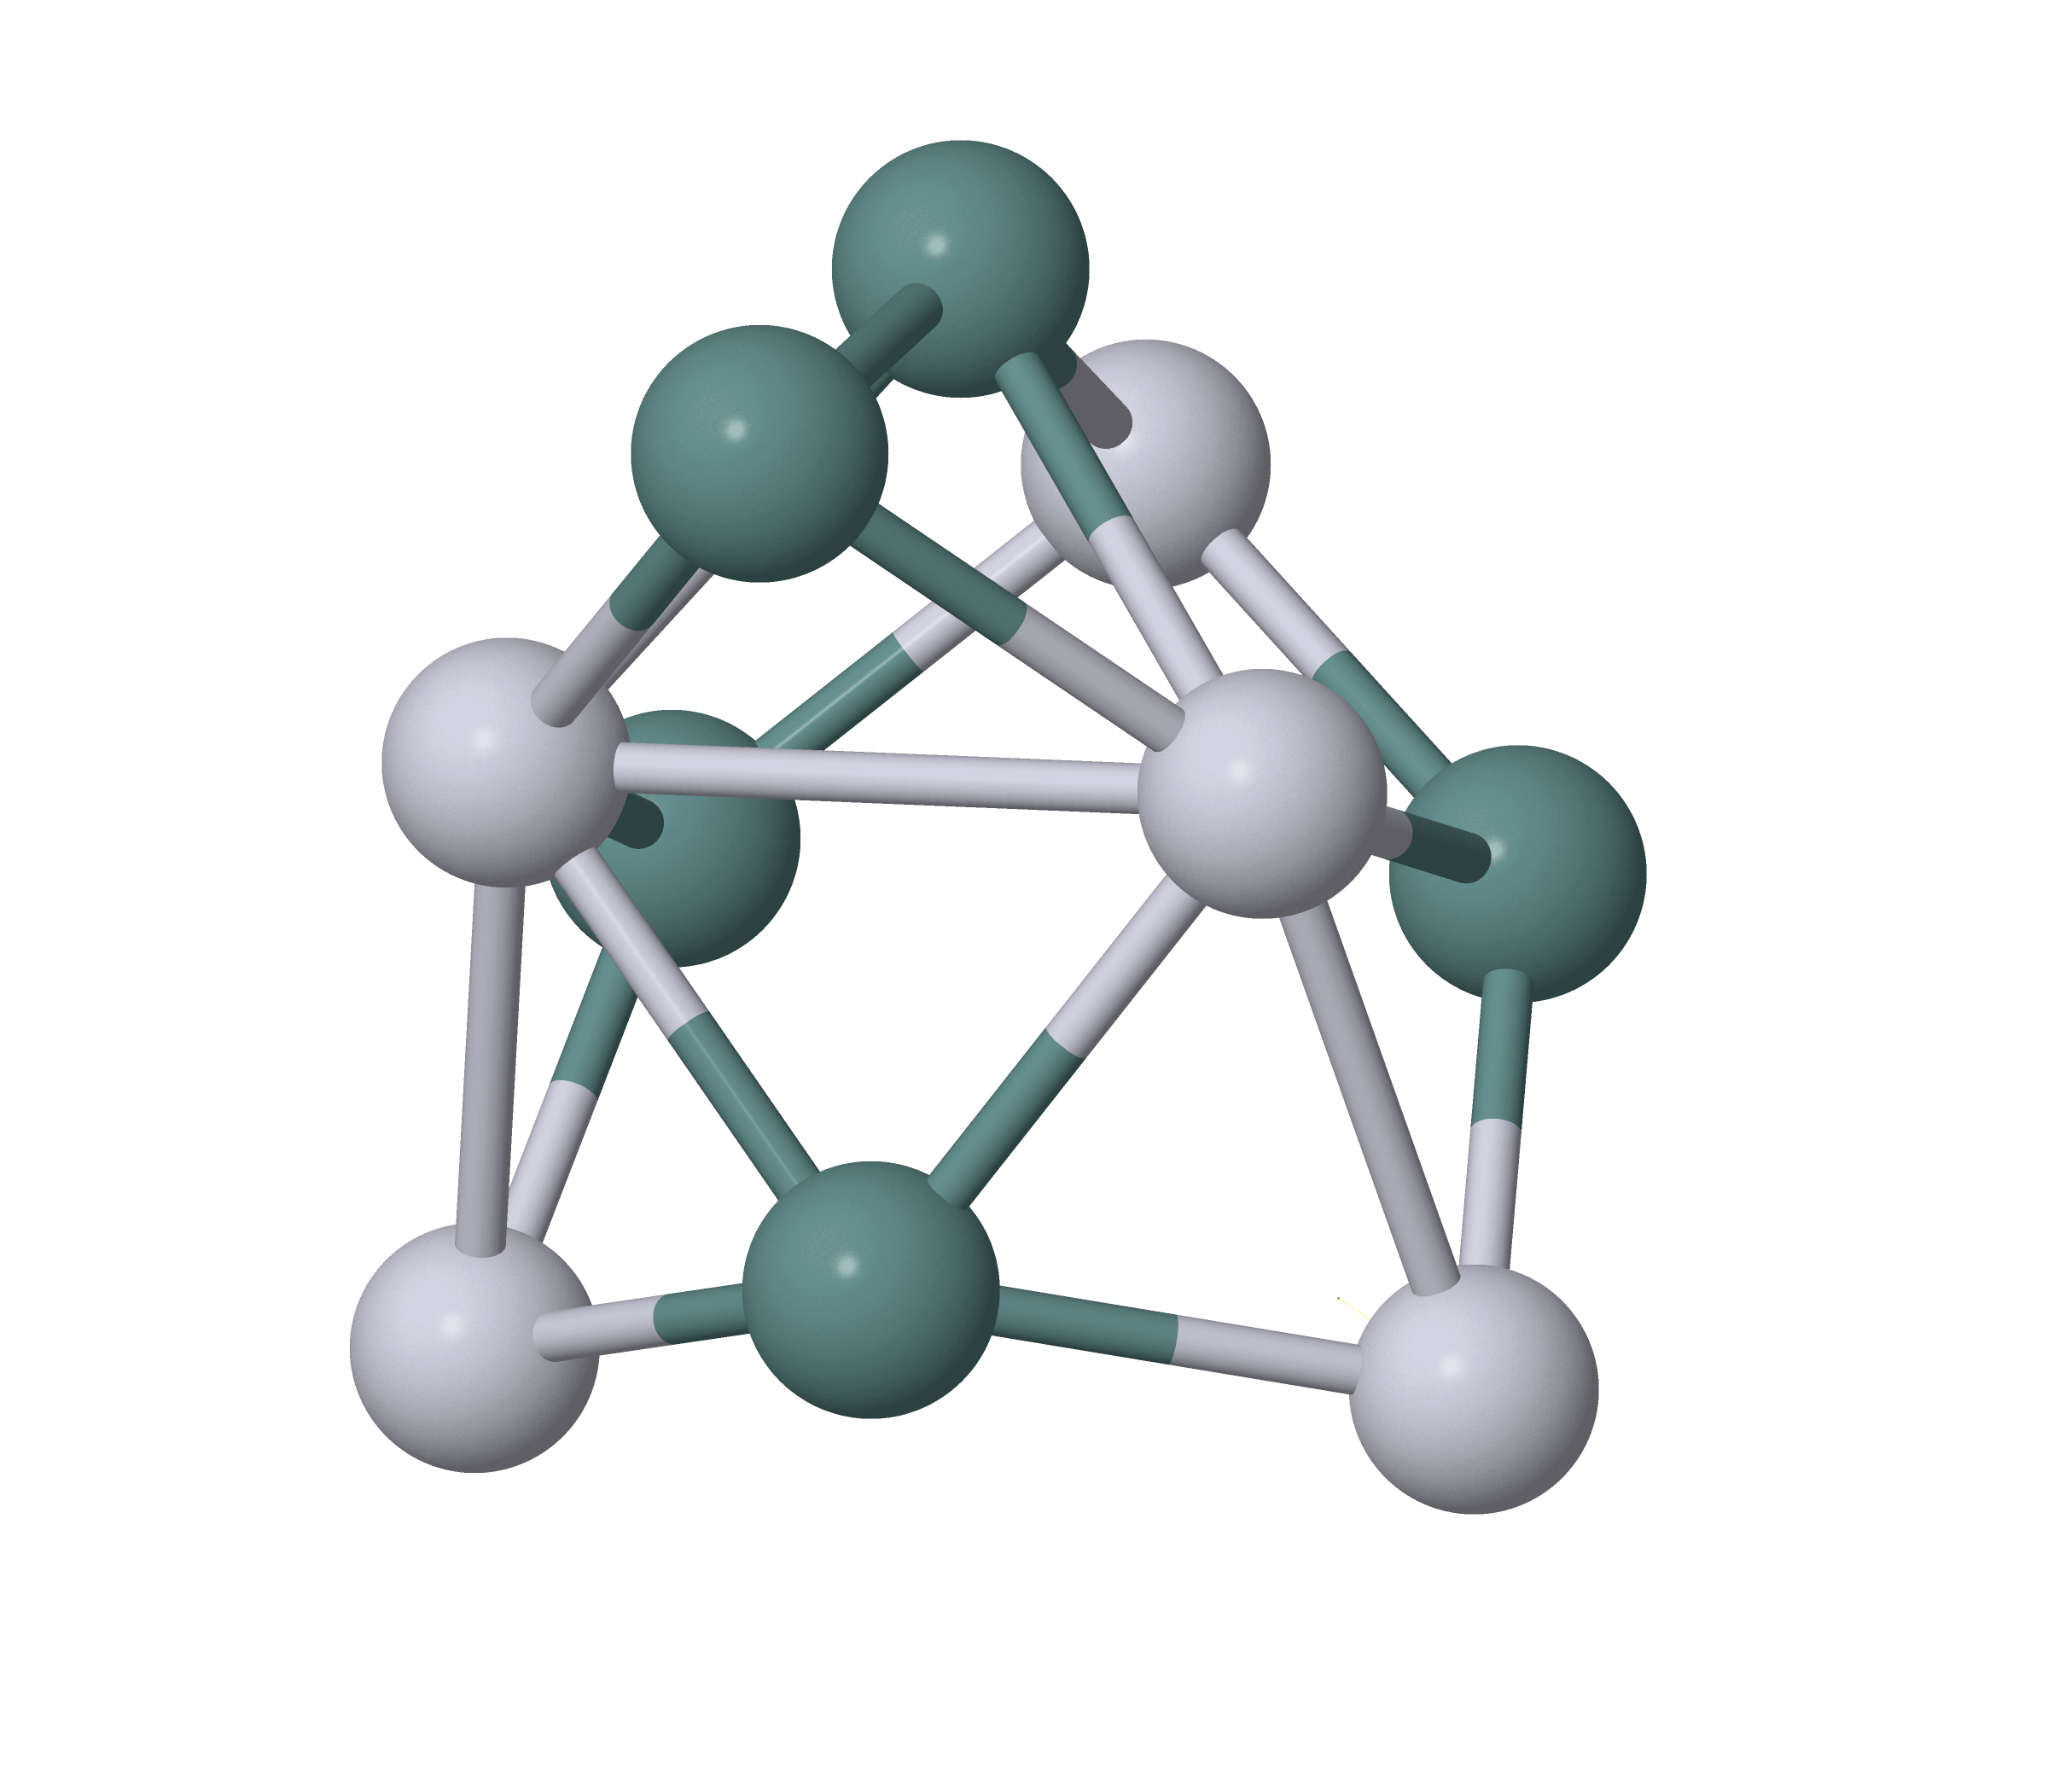
\includegraphics[width=2.10cm]{cluster.png}};
  \node at (1.02,0.40) {$\mathsf{Pt}_{x}\mathsf{Ge}_{10-x}$};
  \node[font=\sffamily\fontsize{12}{13}\selectfont] at (1.97,1.65) {$+$};
  \node[inner sep=0pt] at (2.46,1.65) {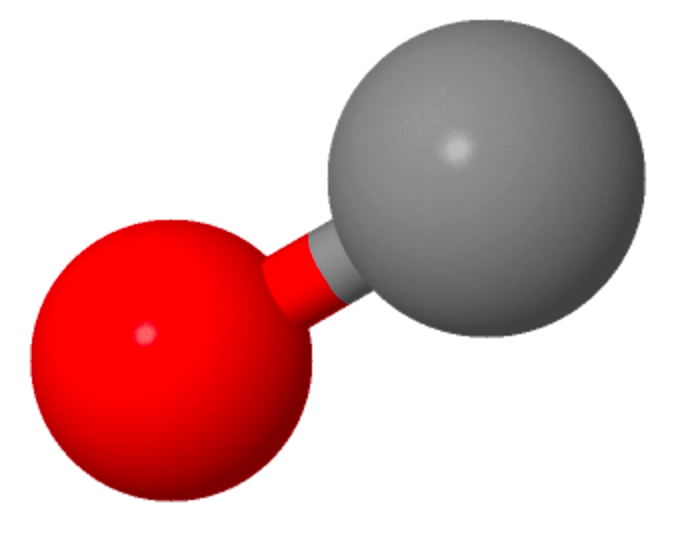
\includegraphics[width=0.48cm]{co.png}};
  \node at (2.46,1.22) {CO};
  \draw[Ink,line width=0.65pt,-{Stealth[length=1.7mm,width=1.1mm]}] (2.88,1.65) -- (3.62,1.65);

  \node[inner sep=0pt] (complex) at (5.15,1.62) {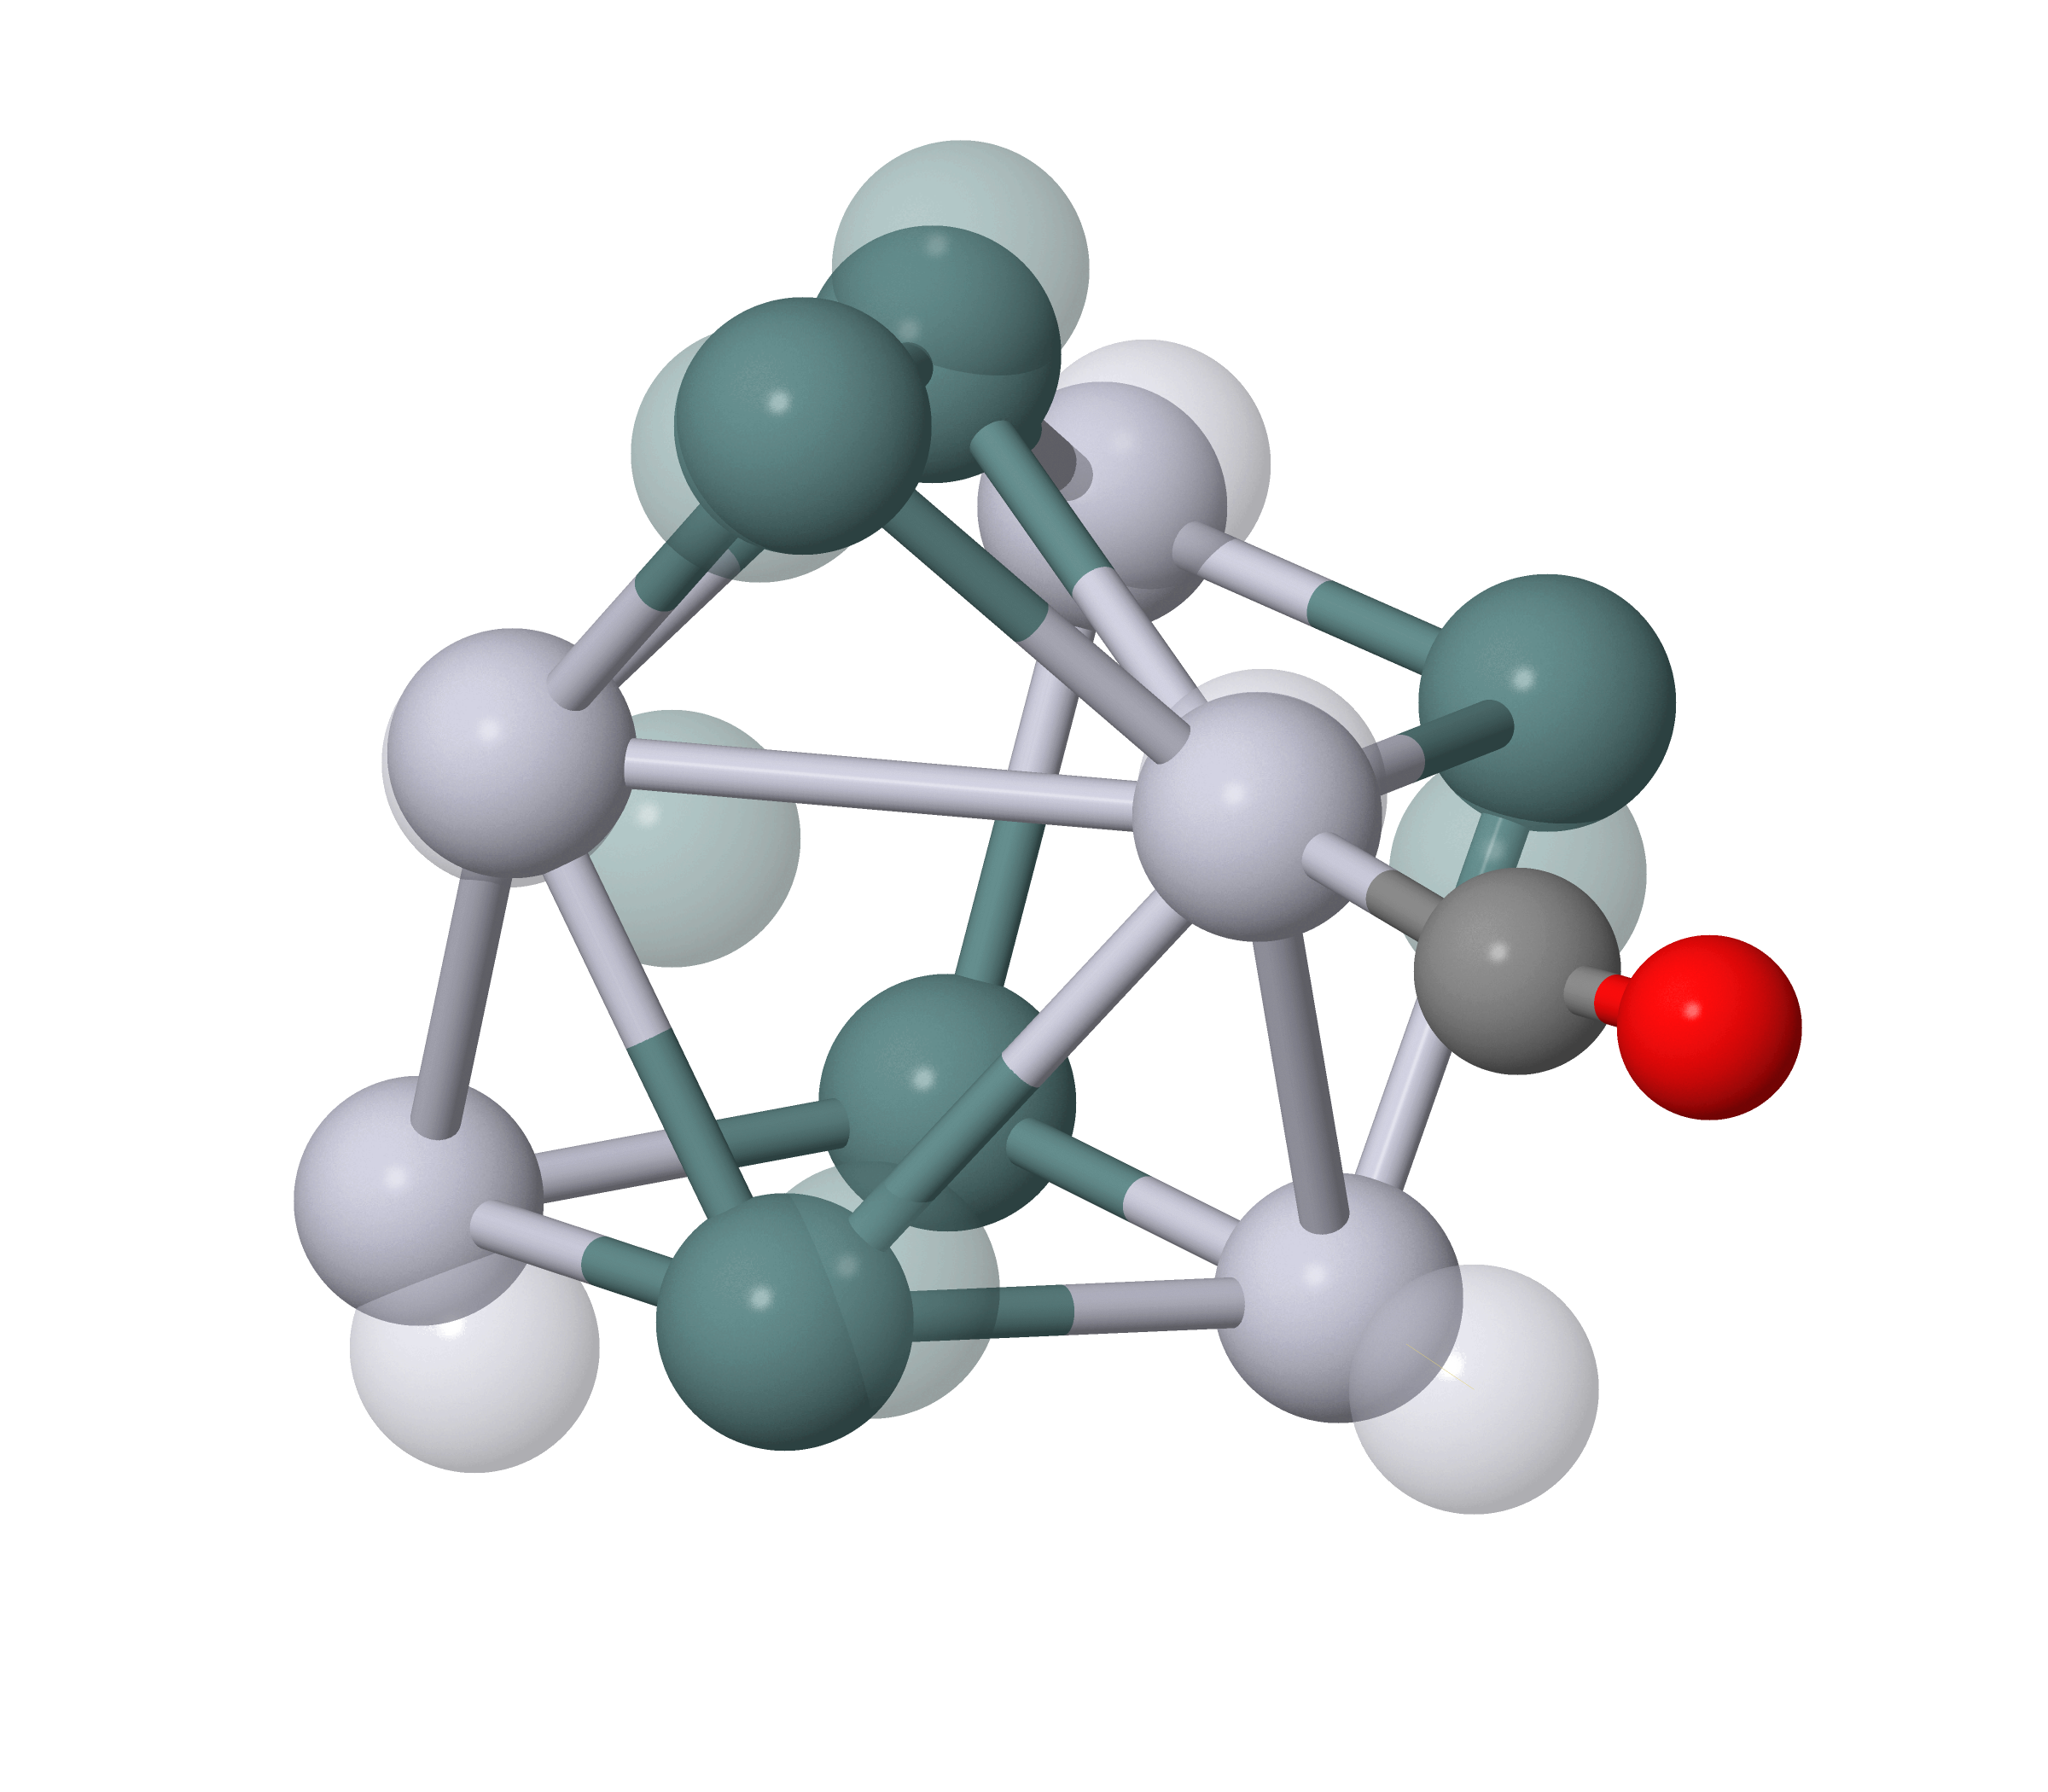
\includegraphics[width=2.90cm]{compare.png}};
  \begin{scope}[shift={(complex.south west)},x={(2.90cm,0cm)},y={(0cm,2.5375cm)}]
    \draw[GeArrow,movement] (0.47,0.90) -- (0.47,0.80);
    \draw[PtArrow,movement] (0.58,0.80) -- (0.55,0.72);
    \draw[GeArrow,movement] (0.75,0.53) -- (0.76,0.64);
    \draw[GeArrow,movement] (0.32,0.54) -- (0.47,0.38);
    \draw[PtArrow,movement] (0.24,0.25) -- (0.20,0.34);
    \draw[PtArrow,movement] (0.74,0.21) -- (0.64,0.30);
    \coordinate (ptcbcp) at (0.674,0.502);
    \coordinate (neighborGe) at (0.75,0.64);
    \coordinate (neighborPt) at (0.57,0.76);
  \end{scope}
  \node at (5.15,0.27) {$\mathsf{Pt}_{x}\mathsf{Ge}_{10-x}\mathsf{CO}$};

  \node[anchor=west,inner sep=1pt] (econlabel) at (6.95,2.43) {ECoN};
  \coordinate (branch) at (6.73,2.43);
  \draw[GeArrow,leader] (econlabel.west) -- (branch) .. controls (6.37,2.43) and (6.26,2.13) .. (neighborGe);
  \draw[PtArrow,leader] (branch) .. controls (6.21,2.43) and (5.77,2.50) .. (neighborPt);
  \filldraw[fill=GeArrow,draw=white,line width=0.3pt] (neighborGe) circle (0.024cm);
  \filldraw[fill=PtArrow,draw=white,line width=0.3pt] (neighborPt) circle (0.024cm);
  \node[anchor=west,inner sep=1pt] (bcplabel) at (6.95,0.97) {$\rho_{\mathsf{BCP}}$};
  \draw[Ink!80,leader] (bcplabel.west) -- (6.78,0.97) .. controls (6.43,0.97) and (6.30,1.47) .. (ptcbcp);
  \filldraw[fill=Ink,draw=white,line width=0.4pt] (ptcbcp) circle (0.03cm);
\end{tikzpicture}
\end{document}
